%% This document gives an example on how to use the ntnumasterthesis
%% LaTeX document class.

%% Use short name MACS, MIS, CIMET, MTDMT, MIXD or MIS  
%% Language english or norsk
%% b5paper with oneside or twoside, you can set A4 if you want but you submit in b5

%% If you want print with the heading material on a4 paper you can use this format
%% \documentclass[MACS,english,a4paper,oneside,12pt]{ntnuthesis/ntnuthesis}

%% with the change to using DAIM we have a new option. include DAIM after english below removes the front page material so that you can then submit in the DAIM system. If you are wanting the front material remove DAIM and make sure you fill in the DaimData.tex file.
\documentclass[MIS,english]{ntnuthesis/ntnuthesis}

\usepackage[T1]{fontenc}
\usepackage[utf8]{inputenc}     % For utf8 encoded .tex files allows norwegian characters in the files. This can be dangerous if you change to a differnt editor.
%\usepackage[pdftex]{graphicx, hyperref}   % For cross references in pdf
\usepackage{graphicx}
\usepackage{hyperref}   % For cross references in pdf

\usepackage[capitalise,noabbrev]{cleveref}

\usepackage{color}              % For colouring text 
\hypersetup{colorlinks=true,     
		linkcolor=blue,          % color of internal links (change box color with linkbordercolor)
    citecolor=blue,        % color of links to bibliography
    filecolor=blue,      % color of file links
    urlcolor=blue           % color of external links
		}
\usepackage{csvsimple}  % for simple table reading and display
\usepackage{url}
\usepackage{booktabs}
\usepackage{gnuplottex} %miktex option if using miktex on windows
\usepackage{rotating}


\definecolor{darkgreen}{rgb}{0,0.5,0}
\definecolor{darkred}{rgb}{0.5,0.0,0}

\lstset{        basicstyle=\ttfamily,
                keywordstyle=\color{blue}\ttfamily,
                stringstyle=\color{darkred}\ttfamily,
                commentstyle=\color{darkgreen}\ttfamily,
}


%Typesetting of C++ but not always stable in titles etc...
\newcommand{\CPP}[0]{{C\nolinebreak[4]\hspace{-.1em}\raisebox{.1ex}{\small\bf +\hspace{-.1em}+\ }}}

%\usepackage[table]{xcolor}% http://ctan.org/pkg/xcolor
%\usepackage[nomessages]{fp}
%\newlength{\maxbarlen}


\newcommand\databar[3][gray!20]{%
  \FPeval\result{round(#3/#2:4)}%
  \rlap{\textcolor{#1}{\hspace*{\dimexpr-\tabcolsep+.5\arrayrulewidth}%
        \rule[-.05\ht\strutbox]{\result\maxbarlen}{.95\ht\strutbox}}}%
  \makebox[\dimexpr\maxbarlen-2\tabcolsep+\arrayrulewidth][r]{#3}}



\newcommand{\com}[1]{{\color{red}#1}} % supervisor comment
%\renewcommand{\com}[1]{} %remove starting % to remove supervisor comments
% This will appear in text \com{Lecuters comment} and be visible unless you uncomment
% the renewcommand line.

\newcommand{\todo}[1]{{\color{green}#1}} % items to do
%\renewcommand{\todo}[1]{} %remove starting % to remove items to do

\newcommand{\n}[1]{{\color{blue}#1}} % other comment
%\renewcommand{\n}[1]{} %remove starting % to remove notes

\newcommand{\dn}[1]{} % add the d to a note to say that you have finished with it.





% Set to true ONLY if using Harvard citation style
\newboolean{HarvardCitations}
\setboolean{HarvardCitations}{false} % false for computer science, true for interaction design and harvard style


\ifthenelse{\boolean{HarvardCitations}}{%
	\usepackage{natbib} % for Harvard names as citations.
}{%
	\usepackage[numbers]{natbib} % for Vancover numbers in bibliography
}

\newcommand{\q}[1]{\leavevmode\marginpar{\small\em #1}}
\renewcommand{\q}[1]{}

\begin{document}

% for students submitting in the DAIM system this information will not be used.
% their is an option for DAIM submission which removes this information and checks it is B5.
% Removing the DAIM option on the document type will use this material.

\setthesistitle{An analysis of on-chain lightning network transactions in the Bitcoin blockchain}
\setthesisshorttitle{On chain lightning network transactions} % a short version for the page headers if your normal title is too long to fit
\setthesisauthor{Jardar Tøn}
\setthesissupervisor{Assoc. Prof. Mariusz Nowostawski}
%\setthesissupervisorA{Prof. Jon Yngve Hardeberg}  % if you have a second supervisor add it like this
%\setthesissupervisorB{Prof. Smart Guy}  % if you have a second supervisor add it like this


\nmtkeywords{Blockchain, payment networks, payment channels, Bitcoin}
%\nmtdesc{This is the short description of a masters thesis}


\setthesisdate{01-06-2018}
\setthesisyear{2018}



%for CIMET theses you need to see all of these as well

%\setthesiscampus{Gj\o{}vik}
%\setthesisHostInstitution{\NTNU}
%\setthesisHostInstitution{University of Eastern Finland}
%\setthesisHostInstitution{Universit\'e Jean Monnet Saint-Etienne}

%\setthesisjuryA{} %jury names
%\setthesisjuryB{} %jury names
%\setthesisjuryC{} %jury names
%\setthesisjuryD{} %jury names


 % this is the file which contains all the details about your thesis
\makefrontpages % make the frontpages
%this is the intro to the thesis
%\thesistitlepage % make the ordinary titlepage
\hypersetup{pageanchor=false}
%\include{summary}

\chapter*{Preface}
This paper is a Master's thesis which was carried out in the autumn semester of 2018 in AIMT at NTNU. The main topics of the thesis is Bitcoin and the Lightning Network, which both are two large systems under active development. Both require a background in computer science for getting a detailed understanding of their operation, but the required background information on both will be provided. This project started as a exploration in the interaction between these systems, which resulted in a approach where the Lightning Network is explored trough the Bitcoin blockchian. While this provided a good scope for the project, the project still had exploratory nature until the first results was produced. 
Even with the bitcoin blockchain as a main approach, implementations for both systems had to be used, and software developed for data collection and processing in relation to both.

%\begin{center}
%\thesiscampus, 
\thesisdate \\[1pc]
\\[1pc]
%\thesisauthor
%\end{center}

\chapter*{Acknowledgment}

I wish first to express my sincere gratitude to my supervisor Mariusz Nowostawski, for his very valuable guidance and support throughout this process. 

I would also like to thank Dmytro Piatkivskyi for his help during the planning and initial stages of this thesis.

A special thanks to my classmates for the time well spent together.

Finally, I wish to thank my parents for their support throughout my study.


\begin{flushright}
J.T.\\[1pc]
\end{flushright}

\chapter*{Abstract}

The blockchain is one of the main mechanisms enabling Bitcoin to be a decentralized electronic payment system. It provides the system with a shared transaction history, which can be verified by every participant. With increased use, it  has become apparent that there is limited possibility for scaling this to handle more transactions. Payment channel networks are one proposed solution to this problem. They allow for more transactions to be done by moving some transactions to a separate network. The Lightning Network is one such network, which uses Bitcoin and the blockchain to operate. While the transactions in this network will not be included in the blockchain, there will be data there related to the network. This is because it needs the blockchain to manage the payment channels which the network consists of. 

In this project we have explored the blockchain with the goal of identifying transactions related to the Lightning Network, and by doing so, determine what information about it is available in the blockchain. We have created different methods for identifying these transactions. The methods use different transaction characteristics differing in uniqueness, making some methods more precise, but having fewer results, and vice versa. We created software implementing the methods, which 
were used to parse the blockchain. The effectiveness of these methods have been quantified by comparing the data we found when parsing the blockchain, to data we collected directly from the Lightning Network. The results shows that the methods are viable for identifying a subset of transactions, and that precision can be sacrificed for finding more.
By identifying these transactions we were able to determine what information about the Lightning Network we can see from the blockchain perspective, and also some aspects where we are limited. 

We have also adapted heuristics from previous work doing blockchain analysis to our scenario.
These were used to link related information we had found when parsing the blockchain, which enabled us to create network graphs showing the relations between the Lightning Network channels identified on the blockchain. While the relations in this network graph were limited, compared to the actual relations found within the lightning network, they show how the blockchain can be used to infer non-explicit information about the lightning network. We have also identified several methods for potentially inferring or locating more information using what is available in the blockchain.

%The Bitcoin blockchian is the public shared ledger defining the shared transaction history for the Bitcoin system. But with the creation of payment channel networks such as the lightning network, the blockchain will also be used to facilitate transactions in a separate network. 
%While the transactions in this network will not impact the blockchain, the channels which this network consists of, does requires the blockchian to operate. These transactions are used to created and close channels, in addition they handle disagreements in the lightning network.
%By exploring the blockchain, we have created methods for identifying the transactions related to the lightning network. The methods use different transaction characteristics differing in uniqueness, making some methods more precise but having fewer result and vice versa.
%The effectiveness of these methods have been quantified by comparing it to data directly from the lightning network. The result shows that the methods are viable for finding a subset of transactions, and that precision can be sacrificed for finding even more.
%By identifying these transactions we have determined what information about the LN we can see from the blockchain perspective, and also where aspects that is limited. We have also adapted heuristics from previous work to these transactions, which we used to link related information. The linked information enabled us to create networks showing relations between the channels in the lightning network. 
%While being limited compared to the actual relations found within the lightning network, they show how the blockchain can be used to infer information about the lightning network. The work also identifies several potential methods for finding more information using what is available on the blockchain.
%
\hypersetup{pageanchor=false}



\tableofcontents

\hypersetup{pageanchor=true}

% Comment with a percent to remove figures or tables:
\listoffigures
\listoftables


\chapter{Introduction}
\label{chap:introduction}

% quick background
Bitcoin is a electronic payment system relying on cryptography and a distributed ledger known as a blockchain \cite{nakamoto2008}. 
It contains all transactions done and is maintained by every node in the network. New transactions is added to the blockchain by spending computational power; making the transactions irreversible as the blockchain grows and more computational power is used, and thus removes the need for trusted third parties to verify transactions. Such a decentralized solution does however not scale well. It can maximally handle about 7 transaction per second \todo{add ref}, compared to visa and other centralized payment systems which can handle ? \todo{ref and numb}.
A proposed solution to increase the capacity and help scale Bitcoin is payment channel networks. Such a network would allow users to do  transactions without them being published in the Bitcoin network and therefore not included in the blockchain which is why they are known as off-chain transactions. This allows for more transactions being done without increasing the capacity of the Bitcoin system itself. It can be thought of as a layer on top of Bitcoin since it require the Bitcoin system and builds on top of it. As the name implies it consist of networked payment channels. A payment channel is a one to one channel allowing the two participants to exchange founds between each other. A network is created by having multiple channels with different users and allowing for transfers to be done across multiple channels-e.g., Alice can pay Bob without having a channel directly connecting them but using intermediary channels. All transactions done inside this network does not impact the Bitcoin network, however the opening and closing of channels does.

%problem description
Because the blockchain is authoritative record of transactions done, because of this property it has been analyzed in research projects \todo{themes of projects and refs}. 
The Lightning Network (LN) as described in the paper by Poon and Dryja \cite{poon2015bitcoin} is a payment channel network currently used with Bitcoin \todo{ref?}. 

%old
The degree of anonymity and privacy users can expect when doing Bitcoin transactions are known from research conducted in recent years.
However, when these transactions are done in the LN, and therefore outside the Bitcoin network there is no longer a clear answer. Since many of these transactions are done off-chain they do not get recorded on the blockchain ledger. This means that we no longer can use the blockchain as a authoritative record containing information on all transactions done. Many of the transaction that used to only be done within the Bitcoin network will now be done in another network entirely. Inside the LN where these transactions are done, people can also transfer founds via intermediaries, which makes it even harder to see the bigger picture of how founds are moving.
Intuitively these off-chain transactions seems to increase anonymity and privacy for the users.
But the details of how this technology effects anonymity and privacy are unknown.

% justification, method 

%old
Many see payment channel networks allowing users to do off-chain transactions as the solution to the scaling issues facing Bitcoin.
But for these solutions to be accepted, the technology and design must be proved to be sound from a security and privacy standpoint. 
In a recent paper on Concurrency and privacy with regards to payment channel networks they also voice this concern \cite{malavolta2017concurrency}. The authors have not found any any comprehensive analysis on privacy, or any analysis that identifies desirable privacy aspects for these types of networks. For the lightning network which is the most prominent example of such a network, it is desirable to resolve potential security and privacy issues while its still under development and few are using it. 


% goals and questions


%old
The notion of anonymity should be well defined, and clear definitions should be established to base the rest of the work on.
Therefore, what are the relevant privacy and anonymity notions in the context of off-chain transactions?

One important aspect of analyzing anonymity in networks such as the LN is determining how the privacy offered by Bitcoin affects the users of the LN. With the blockchain containing a wealth of information can have a large impact on privacy in the LN. What information about the LN and its users can be revealed through data in the blockchain? 

As with other networks the LN will have nodes exchanging data between each other. Therefore, information decreasing anonymity can potentially be found by connecting to the LN the nodes in the network. So, how is privacy and anonymity handled internally in the LN?

We are looking at the problem from two directions: how the LN operates, and the implications of its interaction with the Bitcoin system. When doing this we hopefully get a overall picture of the problem. And we can therefore answer: 
what are the privacy implications of using the LN?

The thesis will find what relevant information is available in the Bitcoin and LN systems, and its impact on anonymity.
Additionally, the methods used to find the information will be outlined, and also how the information is used to assess anonymity.
This will provide a general overview of the anonymity and privacy implications of the Lightning Network.
 % includes latex files from the same directory
\chapter{Background and Related Work}
\label{chap:related}

\section{Related Work}

The work already done on blockchain analysis does not consider the LN as it was done before the LN was conceived of. There is therefore no available work that answers the research question: what information about the LN and its users can be revealed through data in the blockchain?
But the methods used, and how information is deduced from the data contained there can be nevertheless be helpful for this project.
Because the blockchain is a public distributed datastructure containing all transactions done by every Bitcoin user, it is by its nature something that limits privacy. By analyzing the blockchain one can potentially find records of all transactions related to an individual. The amount sent and received, the time and date this was done, and which addresses these transactions was going to or coming from. But as mentioned these addresses used can be generated by users at will. Therefore it is considered best practice to use a new address for each transaction. The result of this is that we have transactions between addresses without knowing which addresses belong to which users. Therefore the goal of the studies who analyzed blockchain data was to cluster addresses used by the same individual, and negate the effect of users creating multiple addresses for different transactions \cite{herrera2015research}, and by doing this also creating user profiles that contain transaction data for that user.

\paragraph{}
One of the first studies which analyzed data from the blockchain to assess privacy was done by Reid and Harrigan \cite{reid2013analysis}.
They used the data to construct two networks, one transaction network and one user network. A Bitcoin transaction stored in the blockchain has at least one input and one output. A output of one transaction will eventually be an input on another. A network created with this transaction data will show how transactions are connected and therefore how founds are moving. The user network tries to link addresses which are likely to belong to the same user. This will create a network were we can see relations between different users. We can also see the transactions were the addresses of a particular user is involved. This clustering of addresses was done in two ways: the input addresses of a transaction with multiple inputs was assumed to be from the same user; the other way was using online sources and online Bitcoin services which had information linking multiple addresses to one user. The review paper by Herrera-Joancomart\́i\cite{herrera2015research} states that this user network model allowed Reid and Harrigan do user centered analysis, and therefore give context to the data in the blockchain.

\paragraph{}
Another paper trying to do address clustering is Androulaki et al. \cite{androulaki2013evaluating}, were they in addition to grouping multiple input addresses for a transaction to the same user, they also utilized the output. Since a single unspent output must be consumed in its entirety by a input for a new transaction, transactions will often generate change. E.g., a user has a 5 coin unspent output available and they are paying someone else 4 coins; the payment transaction will have one output with 4 to the other user, and one output back to the sender with the remaining 1 coin. The address this change is sent to is referred to in the paper by Androulaki et al. as a shadow address. It will not be the same address which was used send the payment but will be a new one belonging to the sender.
To identify which address belonged to the receiver and which is the shadow address they looked at the addresses previously used in the blockchain. The shadow address was assumed to be newly created to receive the change so if one of the output addresses had already appeared in the blockchain they assumed it to be the receiver reusing an address. They also utilized machine learning techniques to further group addresses based on behaviour. They were able to unveil 40\% of user profiles in their experiment. This accurate figure is made possible by having a ground truth, because the data used was from a simulated use of Bitcoin.

\paragraph{}
A more active approach to help clustering addresses is actively participating in the network to collect data, which was used in a study by Meiklejohn et al. \cite{meiklejohn2013fistful}. They participated in mining pools, withdrew and deposited founds on banking services or wallet services, used gambling sites, and purchased goods from vendors. Doing this they could gather addresses and because the addresses collected was certain to belong to a known entity, the tagged addresses would aid clustering in addition to the methods described earlier.
A important remark done both by Meiklejohn et al.\cite{meiklejohn2013fistful} and Reid and Herrigan \cite{reid2013analysis} is that a big entity in the network which does transactions with a large number of other users will have greater opportunity to identify or track users. Such a entity might be a exchange were people trade real money for Bitcoin, in such cases services will most likely have identifying information of users linked to their addresses.

\paragraph{}
In the LN the blockchain is used to open and close payment channels between a pair of nodes \cite{poon2015bitcoin} \cite{malavolta2017concurrency}. These payment channels between nodes form a network which is the LN itself, and were payments can be transferred between two parties without the two needing to have their own payment channel; meaning the payment is routed through the payment channels of intermediary nodes.
Herrera-Joancomartí et al. discusses in their paper \cite{herrera2016privacy} privacy in relation to Bitcoin scaling solutions and also points to several problems with blockhain analysis. One central issue is the sheer size of the blockchain. Herrera-Joancomartí et al. states that at the time of writing that paper the blockchain was 72 GB. The other papers discussed here which did blockchain analysis, did so in 2013 when the blockchain was around 8 GB; now it is over 140 GB \cite{blockchain_size}. 
Herrera-Joancomartí et al. also points out that the clustering heuristics used in previous studies \cite{reid2013analysis}  \cite{meiklejohn2013fistful} are no longer applicable when considering off-chain transactions. Also the transactions themselves that are done off-chain will not be available in the blockchain for analysis. Herrera-Joancomartí et al. suggests that using payment channel networks will increase the privacy of users with regards to blockchain analysis, but that the existing methods may be adapted to analyze the payment channels in a network such as the LN. In the LN paper \cite{poon2015bitcoin} the transaction used to open a channel is referred to as the founding transaction. The output of this transaction is used as input of the transaction closing the channel-i.e., the founding (opening) transaction and closing transaction is linkable. Furthermore, in the LN developer mailing list there is mention of the founding (here referred to as anchor) transaction can imply the network topology \cite{rusty_routing1}. This is because all channels must be anchored in the blockchain with a founding transaction signed by both parties in the channel. This possibility is also mentioned in the LN paper itself \cite{poon2015bitcoin}: by monitoring the blockchain for founding transactions a routing map of can be theoretically built. We do not know whether or not this possibility has been explored any further.

\section{Network Analysis}

There has been no studies doing network analysis on the LN or other payment channel networks.
However, there has been identified several factors in the LN that will impact anonymity.
Herrera-Joancomartí et al. \cite{herrera2016privacy} suggest that the typology of the LN will greatly affect privacy. 
They propose that a possible typology for the LN is one were there are some highly connected core nodes that have big capacity channels with each other, while the end users connect to one of these each when they want to do transactions. In contrast to the Bitcoin network which is a decentralized p2p network, the LN with this topology will be a more centralized one. The number of core nodes and how many connections they have will of course play a big role in the degree of centralization. But any degree of centralization with some nodes being more connected than others will likely have a effect on anonymity. These nodes may be in a position to know both source and destination of payment done in the network. Which violates the privacy notion of relationship anonymity for payment channel networks suggested by Malavolta et al. \cite{malavolta2017concurrency} discussed in section 2.1.
However, onion routing \cite{LN_onion_implementation} has been implemented for the LN which provides relationship anonymity.
In the payment path a node will only know where it received the payment from and where to forward it to. It cannot know if where it received it from was the sender or just another node in the path, or if the next node is the final receiver or just another forwarder. 

\paragraph{}
The mechanism used to transfer the payments over multiple channels in the LN is called Hashed Timelock Contract (HTLC). This contract states that the receiver must supply a preimage (input used in a hash function) to claim the founds from the contract; if this is not done within some time frame the sender will get their founds back. Each node in the path, from the sender to receiver promises to pay the next node by using the HTLC. So, a HTLC between two nodes is created for each hop in the path. The final receiver then discloses the preimage to the node before it in the path, which in turn can now get the founds from the node before it because it now knows the preimage.  This happens until the founds are pulled from the original sender. The term contract is used because if one of the nodes breaches the terms, the contract can still be enforced by using the blockchain to broadcast transaction data and close out the channel to claim the founds. In this manner two parties can transfer founds in a payment path containing untrusted intermediaries. Malavolta et al. \cite{malavolta2017concurrency} points out that this preimage is the same for each HTLC in the path for a payment, it can therefore be used as an identifier among many payments done by the nodes in the network. This means that two nodes can determine that they both where in the path of of the same payment by comparing preimage value. They also suggest that if a node in the path is uncooperative and the HTLC is enforced on the blockchain, the data broadcast there containing the preimage can be used to find the path used for the payment, even without being part of the payment path.

\section{Background}

\subsection{Transactions}

The transactions in the Bitcoin network are how value is transferred between users, but they are also the value themselves.
The coins are more of an abstraction which we can see in Satoshi Nakamoto's definition of a coin: "We define a coin as a chain of digital signatures" \cite{nakamoto2008bitcoin}.
Public key cryptography is used to control transactions; meaning a transaction is tied or owned by a public-private key pair.
To transfer the value of a transaction to another entity, the owner of the key pair locks the transaction using the public key of the recipient, and then uses their own private key to generate a signature showing that the transfer was done by the now previous owner of the transaction. The lock placed on the transaction by the previous owner makes the recipient the one in control of the transaction as they control the private key corresponding to the public one used to lock the transaction. Everyone else  can verify this transfer since the previous owner generated a signature using their private key showing that they had control of the key pair controlling the transaction at the time of the transfer. The datastructure used for transactions represents one transfer of founds from one or more previous transactions; creating a chain of signatures contained in transactions. All previous transactions within this chain can no longer be spent since they have already been transferred, so it is only the tip of the chain which are available to the owner of the key pair controlling it. However, this chain have the ability to fork and merge creating the possibility to split the value of one transaction, or merge the value of many into a single transaction. 
With the possibility of splitting value of a transaction a key pair might not control the entire value of a transaction. We should instead think of ownership of transactions outputs; which together with transaction inputs are the two main parts of a transactions. The output(s) of a transaction is where the creator of the transaction locks the value to a public key, and with multiple outputs can give different keys control of different outputs. Transaction inputs are outputs of previous transactions telling us which value the transaction transfers as shown in fig.\ref{fig:transaction}. As noted earlier, a spent transaction (output) can not be spent again since it is no longer the tip of the chain. This means that if the value given in the input(s) is not used in it's entirety in the output(s) the value missing from the output will be lost. If the creator of a transaction does not wish to transfer the entire value to another entity they can create a output which is locked to their own public key. Similarly there is no output with sufficiently large value for a transfer the sender can crate many inputs from different available outputs to reach the desired value of the transaction. 

\begin{figure}[h]  %t top, b bottom, p page | you can also use h to try to get the figure to appear at the current location
  \centering
  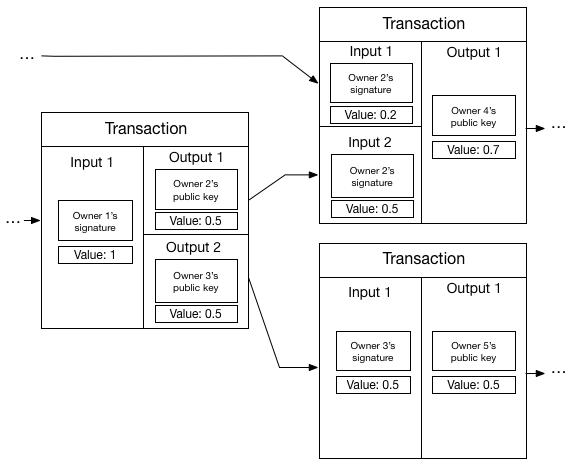
\includegraphics[width=.7\textwidth]{figures/transaction}
  \caption[Transaction chain]{A section of a example transaction chain. We see how outputs of previous transactions become inputs in new transactions and also how transactions can be split and consolidated giving us forks and merges in the chain.}
  \label{fig:transaction}
\end{figure}


\subsection{Blockchain}

The double spending problem is that a user can spend the same value twice, in this case create two transactions, each spending the same output, and both will be valid as the user signed both with their private key; the transactions might be valid but should not be accepted as they spend the same output. To avoid ths in a peer-to-peer system nodes must have consensus about the transaction chain which should be public. The solution Nakamoto \cite{nakamoto2008bitcoin} proposed for creating a shared public transaction history without a central authority, is having nodes timestamp collections of transactions by hashing them together with the previous timestamp hash. 
 The structure containing the transactions at each timestamp is known as blocks, which are published to the network where each node stores their own copy. 
This process of timestamping blocks forms a chain because of the inclusion of the hash for the previous transaction collection, and thereby orders the transactions and proves their existence in relation to other transactions, also validating them futher than just the signature of the owner. A transaction included in a block is proven to have been confirmed by the network and seen as valid at a certain point and spends inputs found in transactions found in earlier blocks in the chain. If someone was to try and double spend an output they would not be able to because only one of the double spending transactions can be included in a block to maintain the integrity of the transaction chain, and if one them was included in a block and thus confirmed the other one will be seen as invalid by all nodes who have a copy of the blockchain and see that this output is already spent by the transaction included in a block. Thus the blockchain ensures consensus by nodes requiring new transactions to spend already confirmed and valid outputs found in a block, and enforcing a common transaction history.

\begin{figure}[h]  %t top, b bottom, p page | you can also use h to try to get the figure to appear at the current location
  \centering
  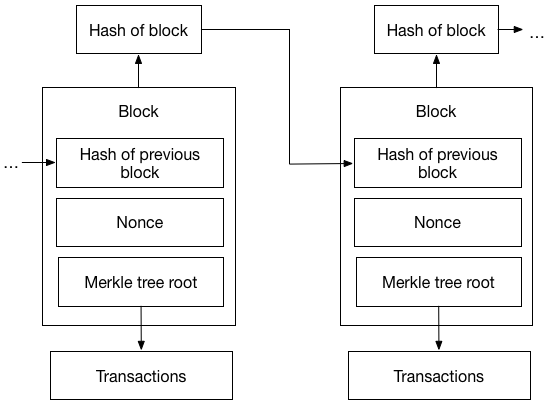
\includegraphics[width=.7\textwidth]{figures/blockchain}
  \caption[Transaction chain]{A section of a example transaction chain. We see how outputs of previous transactions become inputs in new transactions and also how transactions can be split and consolidated giving us forks and merges in the chain.}
  \label{fig:blockchain}
\end{figure}

As new transactions are created they spread around in the network, are validated, and each one node collects them in a pool for transactions that have not yet been included in a block. Nodes try to create blocks by including transactions from the pool and trying to find a nonce to include in the block such that the hash of the block starts with a given number of zero bits. This process is called mining and in addition to awarding new Bitcoin to whoever finds the solution first it requires computational power to be expended for blocks to be created. This system is called proof-of-work because the brute forcing of the hash value requires work to solve; it is also easy for others to verify the solution when the new block is published. As the blockchain grows with more blocks, the total amount of computational resources used increases. This secures the blockchain as it bolsters the immutability of blocks as they get further back from the tip, meaning they will have a greater amount of spent resources on top of them in the chain. As the Bitcoin system is a distributed one, this mining process is how nodes get to vote on their shared transaction history.
To rewrite parts of the blockchain to change the transaction history an attacker would have to redo the work from that point and exceed the height of the current used blockchain. This is because the highest chain is considered the valid one as it has the more work put into it by the nodes. The incentive of new coins when finding a solution and creating a new block also makes spending computational power to change the blockchain instead of mining less desirable. 


\subsection{Transaction Scripts}

Bitcoin transactions use a stateless, stack based, non touring complete language called script \cite{antonopoulos2017mastering}.
The outputs of transactions are locked using script by placing requirements for spending the outputs; inputs contain scripts that meet the requirements placed by their respective output scripts. The language has a predefined set of operations that can be done called Opcodes which limits possibilities of scripts. 
An example of a common locking script placed in outputs is: 
\\

OP\_DUP OP\_HASH160 <receivers public key hash> OP\_EQUALVERIFY OP\_CHECKSIG
\\

This script is a Pay to public key hash (p2pkh) script because the sender can use this script lock the output to the receivers public key hash. The receiver can spend this output by supplying their <signature> <public key> in the input which will meet the requirements placed by the output script and unlock the founds. The unlocking script will be combined with the locking script and executed to ensure that it is valid. 
\\

<receivers signature> <receivers public key> OP\_DUP OP\_HASH160 <receivers public key hash> OP\_EQUALVERIFY OP\_CHECKSIG
\\

The goal of this script is to check if the <public key> in the unlocking part hashes to the <public key hash> of the locking part, and then if the <signature> in the unlocking part matches the public key.
When the script executes the execution pointer will move left to right pushing data to the stack and do the operations specified.
In the case of P2PKH scripts the <signature> will be moved to the stack followed by the <public key>, OP\_DUP duplicates the top item on the stack, in this case the <public key>. Then the OP\_HASH160 will hash the top item of the stack meaning the top <public key>. The <public key hash> given in the locking part of the script will then be pushed to the stack and OP\_EQUALVERIFY will compare the two top items which now are the <public key hash> and the the hash of the <public key> done by the OP\_HASH operation, if they are equal they are both removed from the stack. The final operations OP\_CHECKSIG takes the two last items on the stack <public key> and <signature> and checks them to see if the signature matches the public key which means it was created with the corresponding private key.

There are two "standard" transaction types commonly used; one being pay to public key hash (P2PKH) already described, and the other is pay to script hash (P2SH) \cite{BIP16}. While users are free to create any locking script they wish within the limits of scripts, these types are recognized by most wallet software and allows for senders to transfer value by locking it in known ways. With P2PKH the receiver can just send a hash of their public key and the sender can create the locking script outlined above and just insert the hash. Instead of a public key hash P2SH allows for the same process but with complex scripts by using a hash of the script. A complex script can be created, hashed, and the hash value is used for creating the locking script resulting in:
\\

HASH160 <script hash> EQUAL
\\

The unlocking script will contain the script that was used to create the hash as one stack item only. When this is executed the whole original script, known as the redeem script will be pushed to the stack, then hashed using OP\_HASH, the script hash from the unlocking script is then pushed to the stack, and finally the two hashes are compared.
\\

<redeem script> HASH160 <script hash> EQUAL
\\

This hashing and comparing will ensure that the script supplied must be the original one. After it is confirmed that the given script is the correct one, that script itself is executed to see if it evaluates to true. The conditions for the redeem script must also be satisfied meaning that potential signatures or other data must also be supplied in the input unlocking a output. This "standard" has two executions, one being to check if the redeem script given by the redeemer matches the hash in locking script, and then the redeem script itself is run.
One reason for this is to move the responsibility for supplying these script from sender to receiver. The receiver can create whatever script they wish without the need for the sender to recreate the script when forming the transaction and locking the output. The sender receives a hash of a script and can crate the standard P2SH locking script with the format given above. The receiver needs to know the script to unlock the output but the sender does not need to know the script to transfer value; it therefore makes sense to place the burden of supplying the redeem script on the receiver instead of the sender. A typical use case for P2SH is multisig scripts: 
\\

2 <public key 1> <public key 2> 2 OP\_CHECKMULTISIG
\\

These scripts require multiple signatures to be valid, meaning multiple key-pairs which implies users are required to spend a output.
In the case above two signatures is required for the two keys, indicated by the number 2 before the keys and the 2 after.
This will be the redeem script which is hashed and given to the sender which creates the P2SH locking script for this hash.
The sender does not need to know the public keys required to spend the output or that it is a multisig script in the first place. The receiver however, needs to know as they are the ones who will claim the value and most likely controls (one) of the public keys required in the redeem script.

\subsection{Segregated Witness}

Segregated Witness (segwit) is a change to mainly the Bitcoin consensus layer defined in Bitcoin improvement proposal (bip) 141 and 143 \cite{BIP141}\cite{BIP143}. It changes the structure of the validating data used to verify transactions and where it is stored. As mentioned transactions outputs have a locking script and a unlocking script; the witness is the unlocking script which can be used to check the validity of the output spent. Segwit places unlocking scripts in a witness data structure which is no longer stored inside the transaction it is used to validate. One of the reasons this is done is to fix transaction malleability, which is the ability to change the transaction id (txid) of a transaction. A txid is a hash of all the properties of a transaction including the unlocking script/witness. The only malleable parts of a transaction is the unlocking script, because a transaction is unique and outputs can only be spent once. So if the choice of inputs, choice of outputs, or the value of these changes, it is no longer the same transaction.
Therefore, when the transaction has been created most of it is non malleable, but the unlocking script can be modified in different ways without invalidating the transaction. Adding operations to the unlocking scripts or zero padding numbers used can achieve this effect and change the id while transaction is for all intents and purposes the same \cite{BIP62}. With segwit the txid hash will be calculated whiteout considering the witness data and therefore remove possibilities for malleability. Since the witness data is only used to validate the transaction itself, it is not necessary to determine the state of the blockchain and can therefore become optional for lightweight nodes saving bandwidth. 

Changes in the consensus mechanism within the Bitcoin network could cause the blockchain to fork. If one set of nodes upgrades their software containing other consensus rules they would only create blocks containing transactions following those rules. Similarly the nodes using the old rules will only consider the transactions matching their specifications. The blockchain will thus split from the point which they last agreed on in two different directions each containing their separate transaction history after the split. This is known as a hard fork because of the effects it has on the network and the blockchain. Segwit was designed to avoid this by being backwards compatible with non segwit nodes. Such a change is known as a soft fork since it does not cause a hard fork. Soft forks are easier to introduce to a decentralized network because it does not require a coordinated upgrade of software. A segwit transaction ouptut is constructed such that a non segwit enabled node will interpret the output as being spendable by everyone-i.e., reedemable by a empty signature; this means a non segwit node cannot correctly validate a segwit transaction but will not consider it invalid \cite{antonopoulos2017mastering}. 

Segwit has two "standard" transaction types which mirrors the functionality the existing ones: pay to witness public key hash (P2WPKH), and pay to witness script hash (P2WSH). The main change is how the locking scripts in the outputs is structured; instead of including the script in the output there are now only a version byte with the value 0 to 16 and then 20b bytes representing the public key hash if the output is P2WPKH or 32 bytes of a script hash if the output is P2WSH. Currently only version 0 is used with the rest being reserved for future versions \cite{BIP141}. It is the lenght of the bytes following the version bytes which decides which type of output the script is. A example of a P2WPKH locking script is:
\\

0 <20 byte public key hash>
\\

The unlocking script is found in the witness structure which is a stack containing the required data to validate the transaction.
In the case of the P2WPKH the witness stack will contain two elements: the <signature> and the <public key> which is the same required to validate the older P2PKH transaction type. In the case of the P2WSH type the witness stack can contain a varying amount of items depending on the requirements of the redeem script. If the redeem script is a mutlisig script the stack will contain the required amount of <signatures + public keys> with the last item of the stack always being the redeem script itself.

\subsection{Payment Channels}


The mechanisms for doing exchanges in the channel are simple themselves, but there are many problematic scenarios that can arise when doing off-chain.
A payment channel between Alice and Bob uses 2of2 multisignature Bitcoin transactions. A multisignature transaction means that multiple keys are required to spend a output of a transaction. A 2of2 multisignature means that 2 keys of a potential 2 keys are required-i.e., both Alice and Bob need to use their keys. This ensures that both sides agrees on transactions done with the founds in the channel. Without it, one of them could just create a new transaction spending all founds in the channel, publish it to the blockchain, and thereby stealing from the other.

\paragraph{}
To exchange founds in a channel one first needs to create whats is known as a "founding transaction" or "anchor transaction". Its purpose is to create a common starting point for the creation of new transactions in the channel. The input value of the founding transaction can come from one or both of the parties in the channel, but the output will have a 2of2 multisignature condition. Then a new transaction spending the output of the founding transaction is created which refund the input values of the founding transactions back to its original owners, also with a mutlisignature condition on its output. At this point no signatures for either the founding or refund-transaction has been exchanged, meaning neither of the parties can publish anything to the blockchain. The exchange of signatures is done in a specific order where first the refund transaction is signed by both sides, and only then are signatures exchanged for the founding transaction. The reason for this is to avoid the founds being stuck in the founding transaction because of the multisignature condition on its output. If the founding transaction where published without or before a refund transaction was created and signed, either Alice or Bob could render the founds unusable by not co-operating because of the multisignature condition. After the signatures for the founding transactions has been exchanged it is published to the blockchain. The starting point of the channel is now established; containing the total value available in the channel and also allowing for refunds initiated by either party by publishing the refund transaction.

The transactions describing the balance between Alice and Bob are called commitment transactions. Balance in the context of payment channels is how the total value of the channel will be split between the parties-e.g., the total value of the channel is 10 coins and the balance is 5 to Alice and 5 to Bob; Alice decides to send Bob 1 coin; now the balance is 4 coins to Alice and 6 to Bob; as shown in fig.\ref{fig:ln_commit} where we see the first commitment transaction on the left and the new on the right.

\begin{figure}[h]
    \centering
    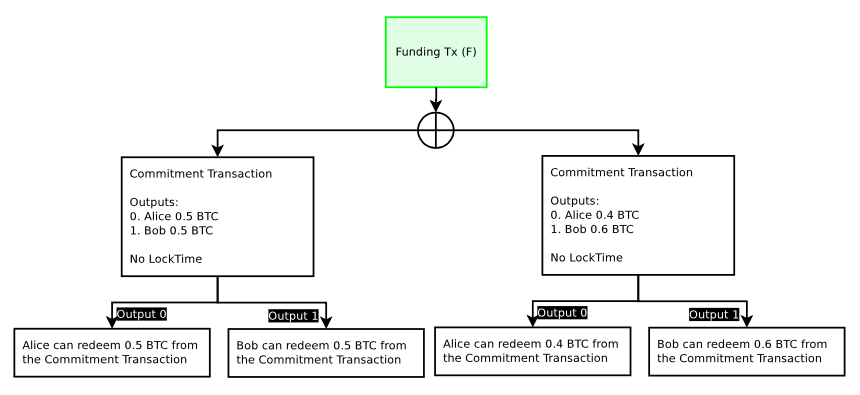
\includegraphics[width=12cm]{figures/ln_commit.png}
    \caption{The founding transaction is colored green to show it has been published to the blockchain. It has two commitment transactions. The leftmost is the original and the right shows the balance after Alice sends Bob 1 coin. Source: \cite{poon2015bitcoin}}
    \label{fig:ln_commit}
\end{figure}

The commitment transactions are all created from the output of the founding transaction just as the refund transaction was. The balance in the channel is described in the output of these transactions, so these commitment transactions takes the total value of the channel in the form of the output of the founding transaction and splits it between the parties in it's own output parameters. The refund transaction can be said to be the first commitment transaction since it describes the initial balance in the channel. This initial balance will be whatever each party contributed to the input of the founding transaction. When the balance in the channel needs to be updated a new commitment transaction is created spending the output of the founding transaction again. The exchanging of founds between Alice and Bob consists of them creating new commitment transactions each time an transfer is done, which represents the new balance between the two. Alice and Bob exchanges signatures for each newly created commitment transaction to satisfy the multisgnature condition, which enables any one of them can publish it to the blockchain at any time they wish. A transaction output can only be spent once, so when a commitment transaction is published the founding transaction is spent, and all other commitment transactions created are therefore useless. This means that the channel no longer has any uses, because its value or founding transaction is spent. So channels are closed out by publishing a transaction spending the output of the founding transaction. Therefore, to be able to do many transfers between the sides in the channel the commitment transactions should not be published immediately. Only when something goes wrong, or both/one of the parties wishes the channel to close should the newest commitment transaction representing the current balance be published to the blockchain. 

The payment channels should not require the parties to trust each other to be able to do exchanges.
As described earlier there are mechanisms that ensures co-operation, such as the refund transaction founding transaction signature order; which makes malicious behaviour such as rendering the founds unusable impossible. A mechanism is needed to solve the big problem of making sure only the newest commitment transaction which has the correct balance is published to the blockcain. Using the earlier example where a channel between Alice and Bob had the value of 10 coins and the balance was 5 to each of them. If Alice Does several payments to Bob and the balance ends up being 0 to Alice 10 to Bob, she could publish the commitment transaction where the balance was 5 to each and get all her money back. To deal with this problem it is proposed to penalize anyone who publishes any other commitment transaction than the latest. The penalty is that whoever published the old commitment transaction will loose all the founds to the other person in the channel.
In order to punish the party who published an old commitment transaction it must be clear which one of them did it; this is known as the problem of ascribing blame. When the two parties exchanges signatures for a commitment transaction we in reality end up with two different versions of the same transaction. Bob signs one and sends it to Alice, and Alice signs one and sends it to Bob. This means both sides ends up with a half signed transaction which only needs their own signature before it is published to the blockchain. The multisignature requirement for commitment transactions means that each side can only publish the one they received from the other.
E.g., if Bob is the one who published a commitment transaction we can find out, because he must publish one of those he received from Alice which already had her signature.

\paragraph{}
The mechanism to punish the party who published an old transaction consists of revoking old commitment transactions. This means each of the parties create a transaction spending their share of a old commitments, signs it and sends it to the opposite party as an insurance. If one side publishes the old commitment  the other will be able to spend the both outputs of the old commitment transactions. This, in combination of enforcing a time period where the person who publishes commitment transactions cannot spend their output, is how old commitments are revoked. So if Bob publishes an old commitment transaction Alice can spend Bobs output before he can do so himself because of the timeout.

\paragraph{}
The timeout of transaction outputs is done with Revocable Sequence Maturity Contracts (RSMC). When looking at the problem of ascribing blame there were two half signed copies of each commitment transaction; Bob got one where Alice has signed, and Alice one where Bob has signed. Both of them are could be published to the blockchain but only the first one will be valid, since they both spend the same output of the founding transaction. The timeout will be placed on the party who publishes the transaction; reason being to try and steal from the other one would publish a transaction themselves-e.g., Alice would publish a old transaction where the balance in the channel favors her and not Bob. For each set of commitment transactions each of them will have a RSMC on the output giving founds to the holder of the commitment transaction. The output which gives founds to the other party is not encumbered with this timeout. Fig.\ref{fig:ln_timeout} shows this structure with two sets of commitment transactions and their outputs. The timeout is enforced by confirmations of the commitment transaction. Confirmations is how deep a transaction is in the blockchain, so when a transaction is included in a block it has one confirmation, when another block is added to the chain it has two and so on\cite{antonopoulos2017mastering}. In the RSMC case it will make the person who publishes the commitment transaction unable to spend their output of that transaction until it has a set number of confirmations. In the paper they uses 1000 confirmations which will take some time when considering a 10 minute block interval.

\begin{figure}[h]
    \centering
    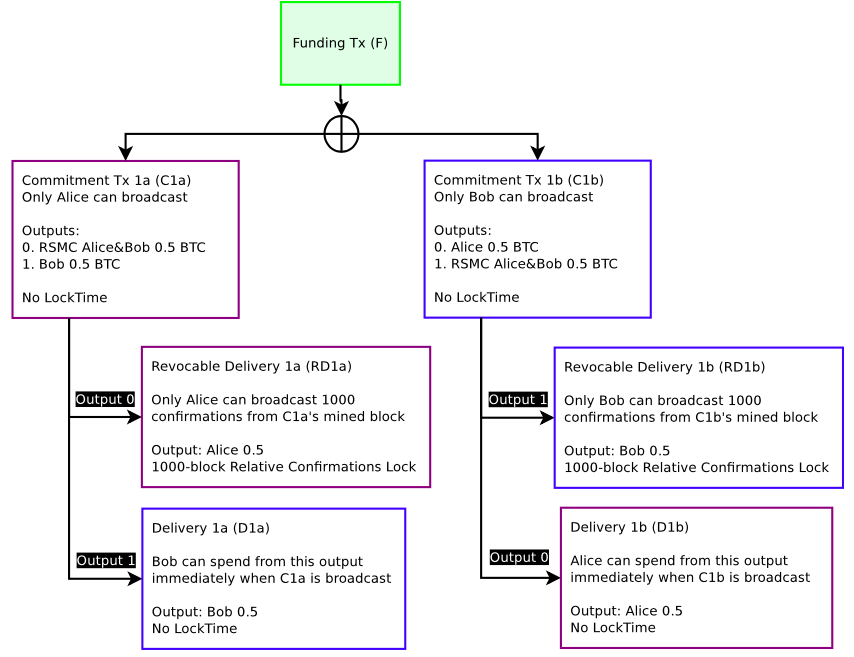
\includegraphics[width=12cm]{figures/ln_timeout.png}
    \caption{Here we see a pair of commitment transactions for Alice and Bob and their outputs. Purple indicates that Alice can publish and blue shows that Bob can publish. Source: \cite{poon2015bitcoin}}
    \label{fig:ln_timeout}
\end{figure}

The need to wait for confirmations to spend the output is something that is enforced on every set of created commitment transactions. It enables the next step that allows for old commitment transactions to be revoked. Whenever a new set of commitment transactions are created both parties sign and exchange whats called a Breach Remedy Transaction. This spends the output that is confirmation locked for that person-e.g., Alice creates a breach remedy transaction spending her output in the old commitment transaction and sends it to Bob. Now if either of the two parties publishes a old commitment transaction, they cannot spend their output at once because of the RSMC, and the other can publish the breach remedy transaction and get their output in addition to their own. The only way one one of the parties can publish an old transaction and get away with it is if the other party does not publish the breach remedy transaction before the timeout is over. If enough time passes so that the commitment transaction gets enough confirmation the one who published it will be able to spend their output as long as the other party has not published the breach remedy transaction. Even so, the other party still would get their output.

\paragraph{}
Lets say Alice and Bob has a channel with the value of 1 coin where they both contributed 0.5 coins each. They create a funding transaction, a refund transaction (which is really the first pair of commitment transactions paying back 0.5 coins to each), sign the refund transaction and then the founding transaction. After the funding transaction is published the channel is ready as shown in fig.\ref{fig:ln_breach}. The current commitment transaction (C1a for Alice and C1b for Bob) have their two outputs giving each 0.5 coins, one normal (D1b and D1b) and one Revocable delivery (RD1a and RD1b) which needs confirmations to be broadcast. Then Alice sends Bob 0.1 coins. Bob creates his breach remedy (BR1b) which spends his 0.5 of the commitment transaction (C1b); this is the same 0.5 output that used in the Revocable delivery (RD1b).
Alice does the same thing and sends it to Bob. Now that the old commitment transactions (C1a and C1b) are revoked they can create the updated pair (C2a and C2b) witch the new balance which outputs 0.4 to Alice and 0.6 to Bob. Now Bob decides to broadcast the old commitment transaction (C1b) to the blockchain. A strange decision since in the old balance he has 0.1 coins less but it's still a violation of the agreement between the parties of not broadcasting old commitments. 
He cannot claim Output 1 of 0.5 coins since he must wait for 1000 confirmations to do so because of the Revocable delivery (RD1b).
Alice sees on the blockchain that an old commitment transaction has been published. She has access to output 0 of 0.5 coins at once since it was Bob who published and therefore there is no confirmation requirement for her. She also has the breach remedy transaction Bob sent her which spends output 1 of 0.5 coins. She can publish this before Bob because he has to wait for confirmations and thereby she gets both outputs and the total value of 1 coin.

\begin{figure}[h]
    \centering
    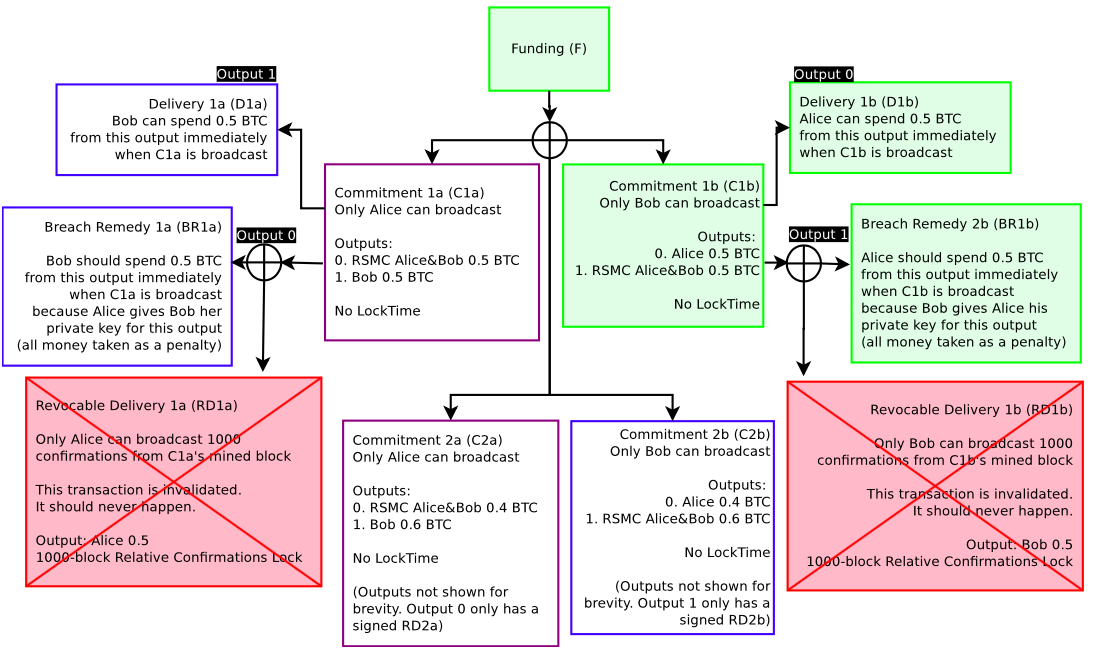
\includegraphics[width=14cm]{figures/ln_breach.png}
    \caption{This is what happens when an old commitment transaction is published. Green indicate that the transaction is published to the blockchain. We see two pairs of commitment transactions, with output transactions shown for the older pair. In this example Bob has published his old commitment transaction violating the agreement, therefore we see that Alice can publish transactions spending both outputs. Source: \cite{poon2015bitcoin}}
    \label{fig:ln_breach}
\end{figure}

\paragraph{}
Publishing a old commitment transaction as described above will spend the founding transaction and close the channel in addition to the other implications already described.
The channel can also be closed out by either of the parties publishing the most recent commitment transaction. If Bob was the one who published Alice can spend her output at once but Bob has to wait for confirmations in the blockchain before he can claim his. But still he will eventually get his output, and since no breach remedy transaction has been made because it is the newest commitment there is nothing Alice can do to stop him from getting his output.
However, the channel can also be cooperatively closed when both parties agrees to do so. They simply create new transaction spending the founding transaction with the outputs reflecting the balance in the latest commitment. They exchange signatures and it can be published on the blockchain. This transaction does not contain any Revocable delivery transaction on its output meaning both will be able to claim their founds at once. 
Another reason for doing this is that the total number of transactions that will be published to the blockchain will be less, one founding and one settlement, instead of the extra revocation transaction.

\section{Networked Payment Channels}

The payment channels discussed in the previous section are for two parties to exchange founds with each other.
As mentioned earlier the LN as described in the paper by Poon and Dryja \cite{poon2015bitcoin} consists of many such channels, forming a network. This means that a user can use this network send founds to others across several payment channels. If everyone needed to create a payment channel with everyone else it would not be very useful, so therefore there are mechanisms such that payments can be routed using other peoples payment channels. Lets say Alice and Bob has a payment channel, but Bob and Dave also has one. Alice wishes to send founds to Dave, and she can do so by sending it first trough her existing channel with Bob, and Bob can use his channel with Dave to deliver him the payment.

As shown in the previous chapter a payment channels used in the lighting network does not require trust between the two parties in the channel. The same should be the case for doing payments across channels without trusting the intermediary nodes along the path. The construction that enables this is called Hashed Timelock Contracts (HTLC).
It works by creating contracts where intermediary nodes have a guarantee that they can get their money from the sender, if they first transfer to the receiver. By having the intermediary first pay the receiver and then get money from the sender one stops the intermediary nodes from stealing the founds. If the intermediary was sent the founds first by the sender they could simply not pay the receiver and keep the founds. But for the intermediary nodes to accept this they need to be sure that the sender will pay them what they have already given the receiver. Using a hash function with an input or preimage R this guarantee can be crated. The receiver inputs R into the function and gets a hash H which is given to the sender. The sender promises to pay the intermediary if they can give R that generates H. The intermediary then promises to pay the receiver if they can provide a R that generates H. Since it was the receiver who created H and therefore has R they can give it to the intermediary and get the founds from them. Now the intermediary knows R and get the founds from the sender as promised.

\paragraph{}
The promise to pay someone in exchange for disclosing R is not only a promise. It is a transaction which needs R to be valid. Therefore when the sender promises to pay the intermediary the sender is no longer in possession of the founds. So the founds are effectively transferred in a manner and direction one would expect (sender, intermediary, receiver) but requires R to be claimed. The timelock is what ensures that if no R is provided the founds can be returned to the one who promised them. It basically ensures delivery of the founds by setting a deadline on providing R. If no such thing existed the series of exchanges could be delayed or stopped by nodes not disclosing R and claiming their founds.
Using an example and figures \ref{fig:htlc_promise} and \ref{fig:htlc_settle} illustrating we can see how this works in detail.
Alice wishes to send founds to Dave, but to do so she must first send them through Bob and Carol. Dave the reciver is the one who creates the hash H with the preimage R and sends H to Alice. She sees that there are tree hops for the founds to reach Dave, so she creates the first HTLC with a three day timelock and sends it to Bob shown as step 1 in fig.\ref{fig:htlc_promise}. To re-iterate the HTLC is a transaction where the preimage R has to be given for the founds to be claimed, if R is not given within the timelock timeframe (three days in this case) the founds can be reclaimed by the creator of the HTLC. Bob creates a new HTLC for Carol with the same condition except that the timelock is two days shown as step 2 in fig.\ref{fig:htlc_promise}. In step 3 Carol creates a HTLC for Dave with the timelock set to one day. At this point the founds have been sent but no one has claimed the founds from the HTLC's so the payment is not complete. If Dave does not disclose R and claim the founds from the HTLC he received it will time out, and so will the other HTLC's.

\begin{figure}[h]
    \centering
    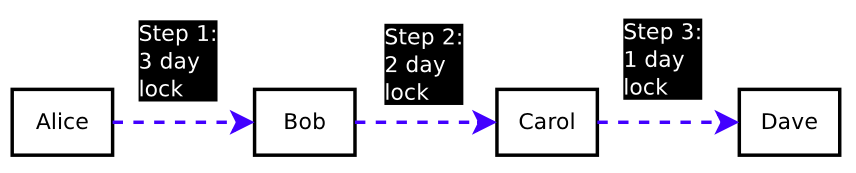
\includegraphics[width=11cm]{figures/htlc_promise.png}
    \caption{ Creating a HTLC between each node with a decrementing timelock. Source: \cite{poon2015bitcoin}}
    \label{fig:htlc_promise}
\end{figure}

In fig.\ref{fig:htlc_settle} we see how the payment is completed with steps 4, 5 and 6 done. Since it is Dave who knows R he must start the process. In step 4 he reveals R to Carol to claim the founds in their HTLC. Carol can then do the same with Bob in step 5, and finally step 6 where Bob can pull his founds from Alice.
Now the founds have been fully transferred from Alice to Dave.
The reason that the timelock must be shorter the closer we get to the final receiver of the founds is because it ensures that each person has time to pull the founds from the preceding one. Lets say that step 3 in fig.\ref{fig:htlc_promise} had a timelock of 5 days, and Dave waited 4 days to disclose R to Carol and get founds from her. The HTLC from Bob to Carol would have expired by then and Bob would have reclaimed his founds, meaning Carol has lost her founds to Dave without any way of getting them back.

\begin{figure}[h]
    \centering
    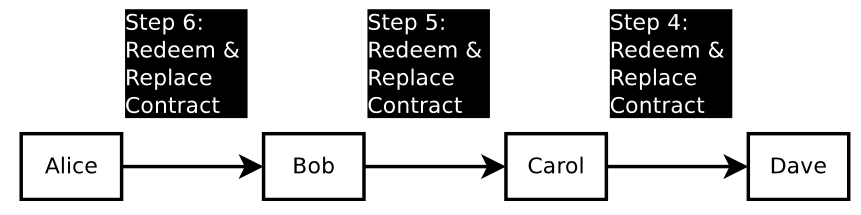
\includegraphics[width=11cm]{figures/htlc_settle.png}
    \caption{ Founds are pulled in reverse order meaning Dave the receiver gets the founds first and the sender Alice looses her's last. Source: \cite{poon2015bitcoin}}
    \label{fig:htlc_settle}
\end{figure}


\section{HTLC inside the payment channel}
The previous section explained how HTLC's can be used to transfer founds across different payment channels.
Here we will show how the HTLC construct interact with the already established dynamic within a payment channel.
A HTLC inside a payment channel will be a output of commitment transactions. Outputs of these commitment transactions reflects the balance between the parties inside the channel, so by having another output we can also reflect founds in transit. The HTLC output is a special type of output; it is a output script which has two different paths to redeeming the output: one is by providing the preimage R, and the other is by waiting for the timelock to expire. As with other output it can only be spent once, and this type must be spent in one of the two ways explained.

\paragraph{}
As an output of commitment transaction the HTLC uses founds available in the channel. If the value of a channel is 10 coins with a 5 to each split, a HTLC for 1 coin will be reflected in the commitment transaction as the sender having only 4 coins, but the total value of the channel will still be 10 (4 sender, 1 HTLC, and 5 receiver). If they both agree on who can spend the HTLC output-e.g., receiver knows the preimage R they can spend. or the timelock is over the sender can spend it, then they can cancel the HTLC and create a new commitment transaction reflecting the new balance. This new balance is either the receiver getting the value of the HTLC or the sender getting it back. This is how HTLC's are resolved off-chain.

\paragraph{}
The two ways of spending a HTLC output is by creating a "delivery" transaction which needs the preimage R to be valid or creating the "timeout" transaction which is not valid until the timelock is gone. If they fulfill their conditions both of these can be broadcast to the blockchain. But since the these transactions spend a output of a commitment transaction the commitment transaction would also need to be broadcast on the blockchain to be able to spend its outputs in new transactions. As explained earlier both parties have the opportunity to broadcast their commitment transaction but restrictions will apply when doing so. The one who published a commitment transaction had to wait before being able to claim their output, while the other party could claim theirs at once. In addition, if the commitment transaction was old and had been revoked by the creation of a superseding transaction spending the
broadcasters output (Breach Remedy Transaction), the other party could use this to get all the founds since the broadcaster had to wait to spend their output.
The same mechanism is used when adding the third HTLC output on the commitment transactions. Using the example of Alice and Bob having a 1 coin channel with a 0.5 to each balance we can see how this works. Alice sends Bob 0.1 coins using a HTLC and they create a new pair of commitment transactions (C2a, C2b) as shown in fig.\ref{fig:htlc_commit} where Alice can broadcast the purple ones and Bob the blue.


\begin{figure}[h]
    \centering
    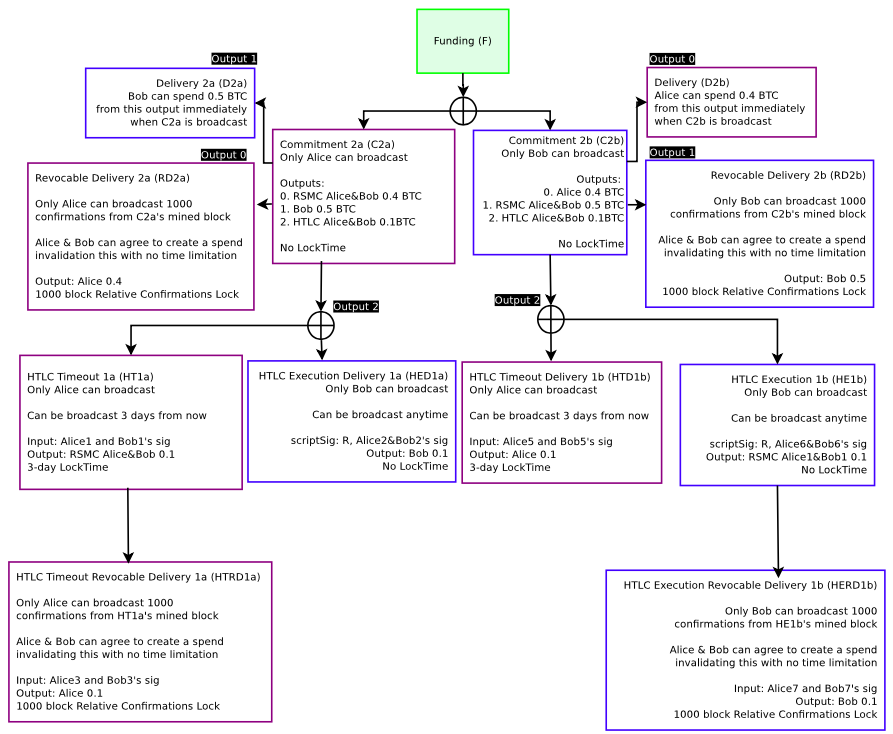
\includegraphics[width=14cm]{figures/ln_htlc.png}
    \caption{ Overview of transactions when including HTLC output to the commitment transactions. Again we have a mirrored structure with the left side showing the case of Alice broadcasting the commitment and the right side Bob broadcasting.  Source: \cite{poon2015bitcoin}}
    \label{fig:htlc_commit}
\end{figure}


\paragraph{}
If the sender, in this case Alice is the one who broadcasts her commitment transaction (C2a) she will have the restrictions placed on her.
In fig.\ref{fig:htlc_commit} this means that the left side will be executed. The commitment transaction (C2a) has three outputs: output 0 is 0.4 to Alice herself (RD2a), but since it is her commitment transaction she will have to wait for confirmations to be able to spend; output 1 is 0.5 for Bob, which he can spend immediately (D2a); output 2 is the HTLC which has two different output paths, Bob can spend at once creating a transaction containing the preimage R (HED1a), or Alice can spend (HT1a) when the timelock has expired but this spend will have a RSMC (HTRD1a) having her wait for confirmations similarly as her normal output (RD2a). This is because similarly as old commitment transactions are invalidated by exchanging breach remedy transactions the same is done by exchanging keys for spending the HTLC output. So if an old commitment transaction is broadcast the party who broadcast will also loose the HTLC output in addition to the normal output, since the other party will be able to spend it and broadcast to the blockchain before the RSMC has enough confirmations. In this case it will enable Bob to broadcast a transaction spending the value of the HTLC before Alice can.

\paragraph{}
In the case of Bob, the receiver broadcasting the commitment transction (C2b), the left side of fig.\ref{fig:htlc_commit} will be executed. We can see that the structure is the same but now Alice and Bob have different restrictions. The output of the commitment transaction remains the same except that now it is Bob who has to wait for confirmations to get his normal output of 0.5 because of the RSMC (RD2b), and Alice can spend hers at once (D2b). In the case of the HTLC output the two parties still have their sender and receiver status meaning Alice can only spend by Timeout of the timelock (HTD1b), and Bob only by providing the preimage R (HE1b). However, since it now was Bob who broadcasted the commitment he is the one who has to get restricted getting the output by waiting for confirmations. So the output of the transaction spending the HTLC output using R (HE1b) is now a RSMC (HERD1b) which will require confirmations to become valid. This is to once again enable the other party (Alice) to get the value in the HTLC if the commitment transaction was an old one.  

\paragraph{}
Similarly as with channel operation without HTLC it is desirable to avoid publishing to the blockchain unless it is necessary. The parties can cooperate and agree on new commitment transactions with or without HTLC outputs. To resolve a HTLC one of the parties must simply prove to the other that they are capable of spending the HTLC output and can do so on the blockchain if they wish. If Bob is the receiver he can publish the commitment transaction and if he has the preimage R he can also create a transaction spending this; because he is the broadcaster he must wait for confirmations on both but will eventually receive his founds. If Bob does not have the preimage R and the timelock has expired Alice can do the same. Since they can prove to the other party that they have this possibility they can instead just create a new commitment transaction pair with the HTLC value either transferred to Bob or returned to Alice, thereby keeping  commitment transactions off-chain and have the channel remain open. When doing this they need to invalidate their old commitment transactions and also the HTLC output of these by exchanging breach remedy transactions and keys. So again we have a system for exchanges between two parties but with the possibility of also using HTLC's which requires no trust, few transactions to be broadcast to the blockchain unless one party is unresponsive or unwilling to co-operate, and allows for founds to be transferred trough many channels.  
When using the HTLC construct to send founds across these channels as shown in fig.\ref{fig:htlc_settle} broadcasting to the blockchain as discussed in this section will ensure the transfer will finish in the event of a node not co-operating as illustrated in fig.\ref{fig:htlc_bc}.

\begin{figure}[h]
    \centering
    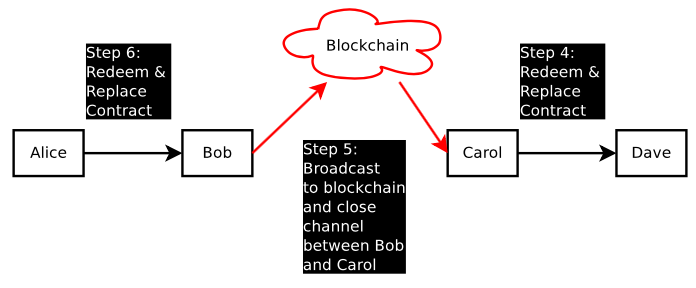
\includegraphics[width=10cm]{figures/htlc_bc.png}
    \caption{ Settlement of HTLC contracts in the event of unresponsive node using the blockchain. Source: \cite{poon2015bitcoin}}
    \label{fig:htlc_bc}
\end{figure} % could be called Methodology or methods or any filename 
\chapter{Methodology and Implementation}
\label{chap:metodology}

Our goal with this project as outlined in \cref{chap:introduction} is creating a method for identifying LN relevant transactions on the blockchain and discover what information will be available to us by doing so. The LN is a separate network but the on-chain transactions it requires for operating channels gives us a link between the two. Because we are interested in what we can learn about the LN and its users from analyzing the blockchain, we will not utilize the information in non LN relevant transactions or users in this project. Reason behind this is the size of the blockchain as discussed in \cref{sec:related}, which means the requirements for both software and hardware will be high if all information should be kept track for parsing. The benefits of taking all information into consideration are also small four our project, however, it can be helpful and is discussed further in \cref{sec:future} on future work. 
\\

The link between the LN and the Bitcoin network will only provide us with a portion of the information about the LN and its users. By connecting to the LN itself we would have access to more information than found on the blockchain. However, the LN is a dynamic changing network of nodes, channels, and payment's; which is not stored in any public ledger like the blockchain. The information found in the LN can be recorded and stored by participants but the system itself does not keep such a record. The data in the blockchain can be verified by any user as explained in \cref{subsec:blockchain} while data recorded from the LN could not be verified in the same manner on its own.
This means that if we want historical data about the LN we must use the blockchain in which the users maintain a consensus about its correctness. Because as already stated the LN requires the Bitcoin system to operate so there will be on-chain transactions on the blockchain. We can also use the fact that there is much information available from connecting to the LN itself: collecting this information will allow us compare it with what we find on the blockchain. Doing this comparison we can verify our method for identifying LN relevant transactions on the blockchain. 
In this project we have created a method for identifying LN relevant transactions while parsing the blockchain, collected data from the LN to compare to the blockchain data, and applied methods for linking relevant information to reveal non-explicit information. 
%analysis of anonymity include.

\section{Blockchain analysis}

The transactions in the blockchain is linked with outputs - inputs forming a DAG as we explained in \cref{subsec:transactions}. Parsing the blockchain would entail linking these transactions to form a transaction graph. When applying the heuristics used by previous works discussed in \cref{sec:background} one can use the information discovered there to provide context to the graph. In our work we do not create a complete transaction graph; we only link transactions related to a single LN channel which gives us a set of sub graphs of the complete transaction graph, each representing LN a channel. Only creating these small sub graphs is considerably easier because we do not need keep track as much data when the parsing is done. To create these graphs we must first differentiate between on-chain LN transactions and normal Bitcoin transactions.
\\

To locate LN relevant transaction on the blockchain we identified attributes they contained not present in other transactions. As stated in \cref{subsec:pcln} Lightning channels have two main on-chain transactions: the founding/opening and closing transaction as seen in \cref{fig:ln_tx_graph} with the two middle transactions. The founding transaction will contain the channel output, and the closing transaction will have the channel input. This output - input pair will be of the type P2WSH 2of2 mutlsig as stated in \cref{subsec:pcln}. This will be the case for all output - input pairs used for these on-chain transactions, but it is not sufficient to determine if a transaction is related to the LN or not, because P2WSH 2of2 multisig transactions can be used for other purposes. As we explained in \cref{subsec:scripts} a P2SH (non segwit version of P2WSH) lock type will only have the hash of the script in the output, while the redeem script itself is included in the input of the spending transaction. This means that if we only consider a founding transaction output we will only be able to tell if the output is a P2WSH type, but if we only look at the closing tx input we will be able to tell that the type is P2WSH and that the redeem script is a 2of2 multisig script. Since both properties must be present in a LN channel output - input pair, we can say that it is more likely the transactions containing the inputs is relevant to LN based on the closing transaction rather than the founding tx. While this method cannot determine if transactions is related to the LN or not, it allows us to say that the transactions types in question are likelier than others to be LN related. We will discuss identification using this method later in this chapter.
\\

In addition to 2of2 multisig redeem scripts there is other script types used in certain LN on-chain transactions. One of these scripts is the one used when a channel is unilaterally closed-i.e., one of the parties in the channel publishes a commitment transaction. As explained in section \cref{subsec:pcln} the one who publishes a commitment transaction has their output of the commitment timelocked; this is to enable punishment for the publisher if the commitment in question was a revoked one with outdated balance favoring the publisher more than the most recent commitment. As stated in the LN specification \cite{bolt3} this unilaterally published commitment transaction has two outputs: one P2WPKH to the party who did not publish, and one P2WSH output with a redeem script which can be spent by waiting for the timelock it contains or with a revocation key. 
This redeem script is fairly unique and to our knowledge there is no other instances such scripts are used. However, people are free to create such scripts without it having anything to do with the LN, but the specific use case of such script makes this unlikely. Because the redeem script is located in the transaction spending a P2WSH output, we need for this case locate it in the transaction spending the timelocket output from the closing/commitment transaction. We will refer to this as the timelocked transaction which is shown on the right in \cref{fig:ln_tx_graph}. Since transactions have references to previous transaction hashes \todo{check if transaction hashes is explaned in bckground} we can by finding the transaction spending a timelocked output get the hash of the timelocked tx. When we have the timelocked tx it will contain the hash of the input tx, and this will again allow us to find the tx hash of the closing tx which will in turn give us the founding tx. Doing this will result in us finding all on-chain transactions related to a unilatirally closed lightning channels.

\begin{figure}[h]
    \centering
    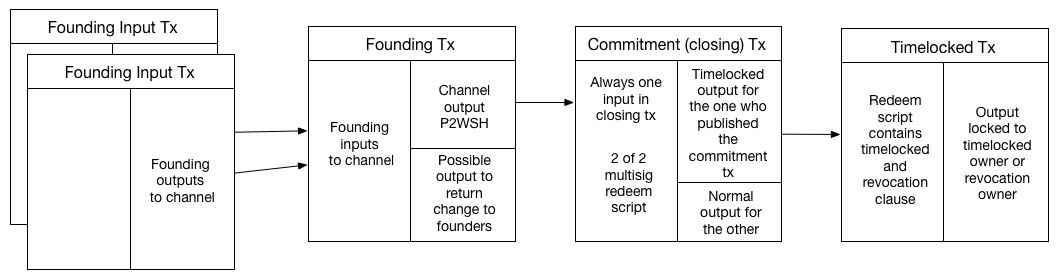
\includegraphics[width=14cm]{figures/ln_tx_graph.png}
    \caption{Transaction subgraph of unilaterally closed channel}
    \label{fig:ln_tx_graph}
\end{figure}


This method identify the transactions related to a lightning channel in reverse order meaning the transaction spending the timelocked output will be indentified first and the founding transaction last. 
This means we must parse the blockchain in reverse order starting from the lastest block working our way down the the start; the structure of the blockchain with blocks only contain the hash of the previous block is another reason for this.
For this project we have developed software parsing the blockchain and identified relevant transaction as outlined above.
At a high level the software finds the top block from the chaindata stored in the database and uses it as a starting point.
Then it traverses the transactions in the block and checks if they are relevant for our project, if that is the case they are stored for later use. The hash of the preceding block is used to get it from the database and same process is repeated.
The algorithm used is based on identifying scripts from the timelocked output of a unilaterally closed channel, and then using the transaction hash of the previous transaction to get the rest of the relevant channels as shown in fig. \todo{add ref fig}

\begin{figure}[h]
    \centering
    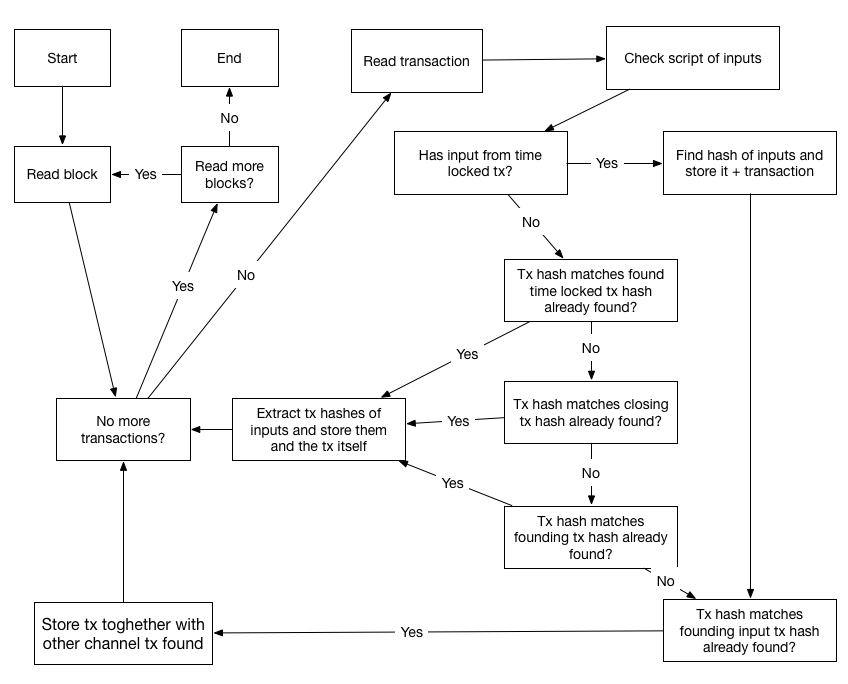
\includegraphics[width=14cm]{figures/algorithm.png}
    \caption{Algorithm of parsing and locating relevant LN transactions on the blockchain}
    \label{fig:htlc_bc}
\end{figure}

% ln transaction formats on chain

When a transaction is inspected we first check if it has a input containing a redeem script for a timelocked transaction.
The script is defined in the lightning rfc \todo{add ref to rfc} and has the format:
\\

\noindent OP\_IF \\
    # Penalty transaction \\
    <revocationpubkey> \\
OP\_ELSE\\
    `to\_self\_delay`\\
    OP\_CSV\\
    OP\_DROP\\
    <local\_delayedpubkey>\\
OP\_ENDIF\\
OP\_CHECKSIG\\

The first line is the clause to stop participants from publishing old commitment transactions. The script will evaluate to true if this clause is used and the signature for the public key is given; As discussed in section \todo{ref bacground} the parties will revoke old commitment transactions by exchanging keys so the other party can spend the timelocked output with the revocation key and get all the founds in the channel. The else clause is the timelocked portion of the script; it will contain a delay and the CHECKSEQUENCEVERIFY operation defined in \todo{ref bip 112} which terminates the script if the delay has not passed. The delay is then removed from the stack with OP\_DROP such that the signature and public key are the only two items on the stack when OP\_CHECKSIG is used to very the signature.

% identifying scripts in depth

% multisig detection

% how other information gathered. output types so on.

\section{Lightning network analysis}

% lnd introduction

%why gather ln data (relate to background and goals)

%how ln data was gathered

To gather data from the LN we used a modified version of the LND \todo{add ref} implementation, which follows the BOLT specification \todo{add ref}. It maintains a view of the network by storing a graph containing active channels. This is continuously updated as new channels are annouched and closing transactions is found on the blockchain. It requires a bitcoin backend running to interact with the bitcoin network; using it to publish on-chain transactions and monitor the blockchain. New channels are discovered by annouchements within the LN while channels closing is found by looking at the blockchain and finding transactions spending the founding transactions of previously active channels. We forked and modifed LND to create a copy of its database each time a new block notification was received from the Bitcoin software giving us a snapshot of the network on each new block.
\\

Each snapshot we collected contained the graph describing the network in its current state, so by comparing the graphs of different snapshorts we can see how the network evolves over time. When comparing two snapshots from two points in time we can identify closed channels by checking the old snapshot for channels not found in the new one; Similarly new channels can be found by checking the new snapshot for channels not found in the old one. This allows us to build a list of closed and opened channels during the collection timeframe, as well as the those which are open throughout. 

% details getting channels.

% comparing to blockchain data

\section{Clustering}

% intro clusting, goals and related work

% how we cluster channels and so on. % could be results
\chapter{Results}
\label{chap:results}

In this chapter we will present the results of applying the methods discussed previously to the data in the blockchain and data we have gathered from the LN. Bitcoin has a testnet used for development and experimental functionality in which the LN have been tested for longer than it has been used on the mainnet. We have used both the testnet and the mainnet in our project; our reasoning for this is the LN on the testnet is bigger, and people are testing a wide array of use cases and functionality using testnet coin without any value; while on the mainnet users have to use Bitcoin with value, but this can result in more realistic user behaviour which impacts the data generated.
By using both Bitcoin networks we will have one with more edge cases and more data, and one containing data reflecting real user behaviour.
The testnet has its own blockchain as the mainnet and is therefore publicly available in the same manner. Collecting data from the LN as we discussed in \cref{sec:ln_analysis} was done in two intervals of one week each. Creating a snapshot of the network on each block for a week results in about 1000 blocks worth of data. This should be sufficient to verify our methods of identifying relevant LN transactions, but doing this twice also allowed us to make adjustments after the results of the first interval.

\section{Method verification with LN data}

Comparing data from the LN with our data from the blockchain provided us with results about the extent our identification methods was able to locate LN channels on the blockchain and to which degree. There is three sets with data was used in these comparisons: 
\begin{itemize}
    \item The set \( \alpha \) , counting channels from the LN closed during the capture interval. 
    \item The set \( \beta \), containing channels from the blockchain identified using timelocked redeem scripts,
    \item The set  \( \gamma \), containing potential channels identified on the blockchain using 2of2 multisig scripts.
\end{itemize}

As we stated in \cref{sec:bc_analysis} and \cref{subsec:pcln} a LN channel uses the P2WSH 2of2 multisig type for the on chain founding - closing output - input pair, and we discussed how this could be used to give us a set of potential transactions being related to LN channels by discarding other types of transactions. Because the on-chain channel transactions must be of this type the \( \gamma \) set is guaranteed to include all channels closed in the block interval used for the search. It also means that the two other sets will be subset of \( \gamma \). So the relations between the sets should be as follows:

\begin{equation} \label{eq:1}
      \alpha \subseteq \gamma, \hspace{10pt} \beta \subseteq \gamma, \hspace{10pt} \beta \subseteq \alpha  
\end{equation}

The two first relations is explained above and is always true for the systems in its current case. The last relation however, will not hold with our data, but ideally it should be true. For this to be the case our method with timelocked redeem scripts for identifying channels should not have any false positives-i.e., identify channels which is unrelated to the LN. We should also be able to discover all closed channels from the LN during the interval, so we get the complete set of actual channels-i.e., \( \gamma \) contain all LN channels closed in the interval. While the timelocked scripts are very unique and therefore good for identifying channels, and theoretically one could synchronize and get all LN channels through the network, this would only always be true in a ideal world scenario. So as we will see with our data \( \beta \not\subseteq \alpha \), but keeping the relation in mind will be useful when analyzing the data.

\subsection{First Interval}

\begin{figure}[h]
    \centering
    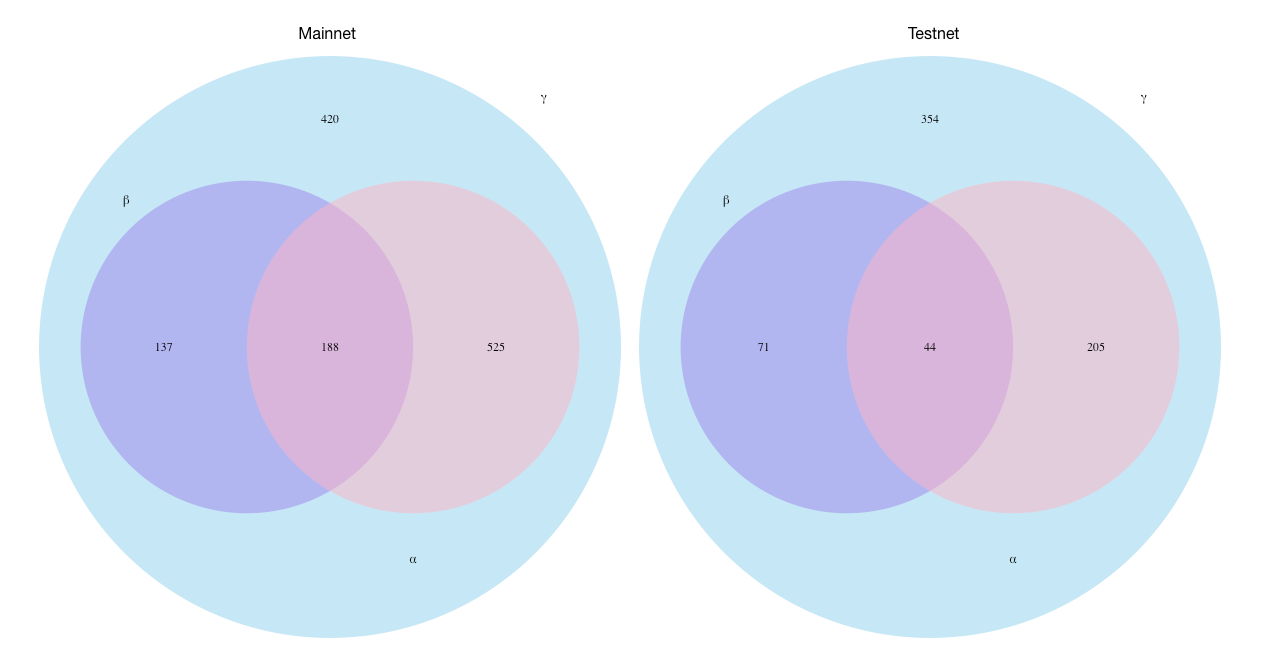
\includegraphics[width=16cm]{figures/graphs/venn_full1.png}
    \caption{Venn diagram of channel sets in interval one}
    \label{fig:venn_run1}
\end{figure}

The first interval for the mainnet had a length of 1151 blocks between block 517855 and 519005. Our modified LND implementation described in \cref{chap:metodology} collected data from the LN and produced the set \( \alpha \) containing 713 channels which where closed during this interval. The same interval on the blockchain was parsed two times, once identifying channels using timelocked redeem scripts, and a second time getting all potential channels using multisig identification. This resulted in a \( \beta \) set containing 325 channels and a \( \gamma \) set with 1270 channels shown on the left left in \cref{fig:venn_run1} as a venn diagram. We can see how both \( \beta \) and \(\alpha\) is a subset of \( \gamma\), but \(\beta \not\subseteq \alpha\). The intersection \(\beta \cap \alpha\) is the number of channels we identified using the timelocked method which was also found trough the LN node. On the mainnet this intersection was 188 which is 26.37\% of total channels in \( \alpha \). This is reasonable as the method will only discover a channel if it has been unilaterally closed as we explained in \cref{sec:bc_analysis} and not if a channel is closed cooperatively which likely will happen more frequently. We should also note the large \( \beta \backslash{} \alpha \) relative compliment of \( \alpha in \beta \) is 137 which is 42.15\% of of the channels in \(\beta\). Having a false positive this high is very unlikely because the uniqueness of the timelocking redeem scripts, so we made the assumption that these are actually LN channels which we have not been able to capture in our interaction with the LN. \todo{add for interval 2 more peers}
This means we can assume the union \(\alpha \cup \beta \) are all LN channels, which would mean the total number of LN channels closed in this interval is 1038. The potential multisig 




\subsection{Second Interval}


\begin{figure}[h]
    \centering
    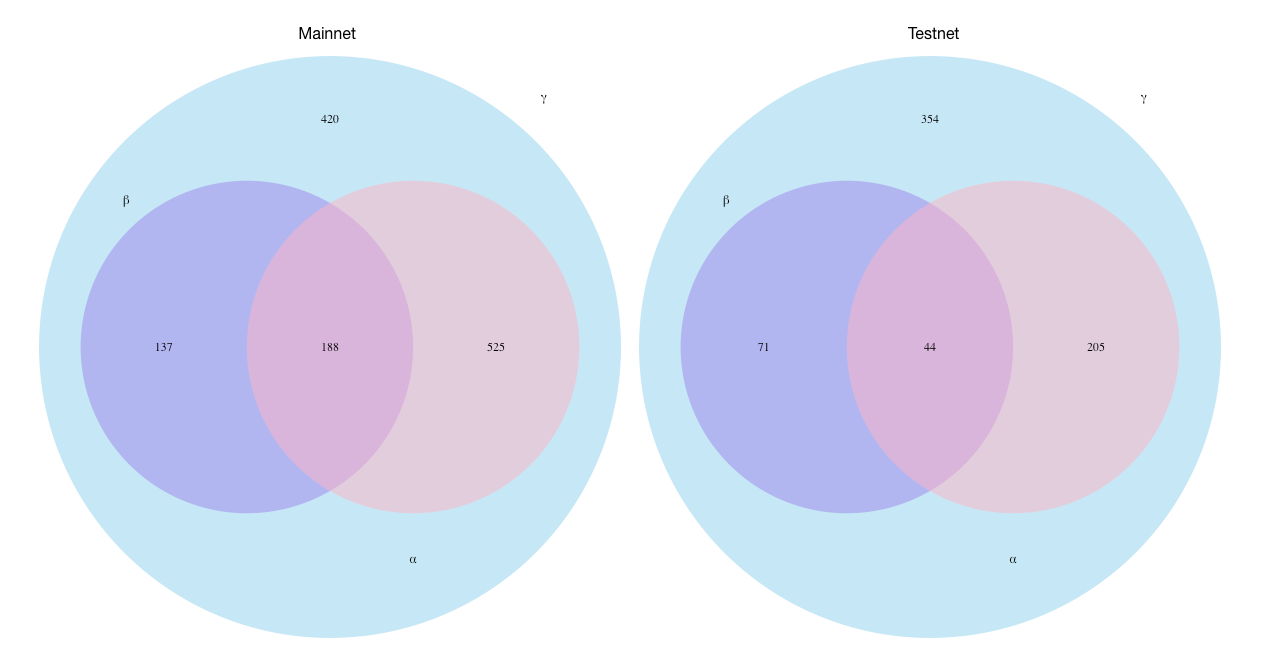
\includegraphics[width=16cm]{figures/graphs/venn_full1.png}
    \caption{Venn diagram of channel sets in interval one}
    \label{fig:venn_run2}
\end{figure}



\section{LN size}

\begin{figure}[h]
    \centering
    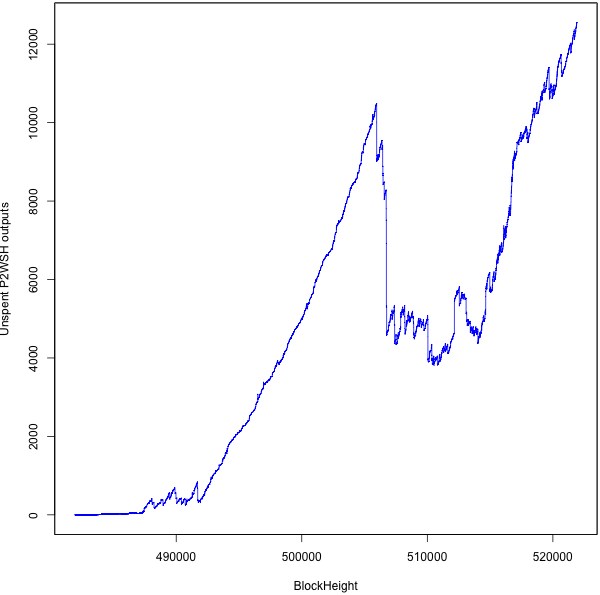
\includegraphics[width=10cm]{figures/graphs/lnsize_mainnet.png}
    \caption{Maximum size of the LN based on unspent P2WSH outputs on the blockchain}
    \label{fig:htlc_bc}
\end{figure}

\begin{figure}[t]
    \centering
    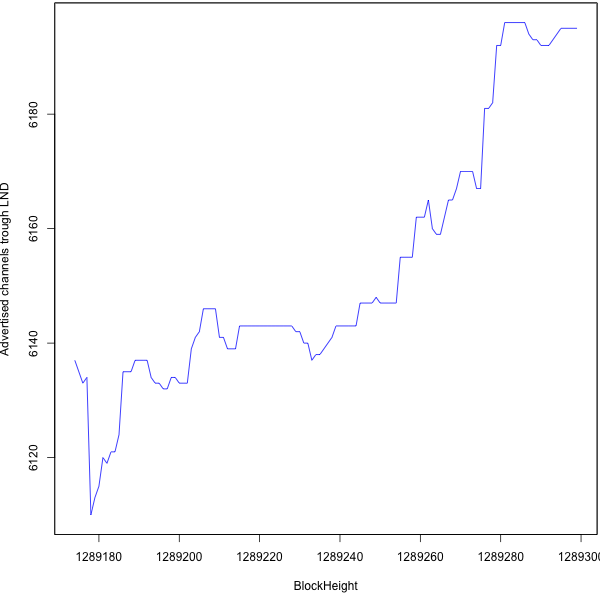
\includegraphics[width=10cm]{figures/lnsizeTS.png}
    \caption{Channel count from LN on testnet}
    \label{fig:htlc_bc}
\end{figure}


\section{Other metrics}

% single founded vs multiple founded txs.
% channel size
% channel lifetime

\section{Clustering}

\begin{figure}[h]
    \centering
    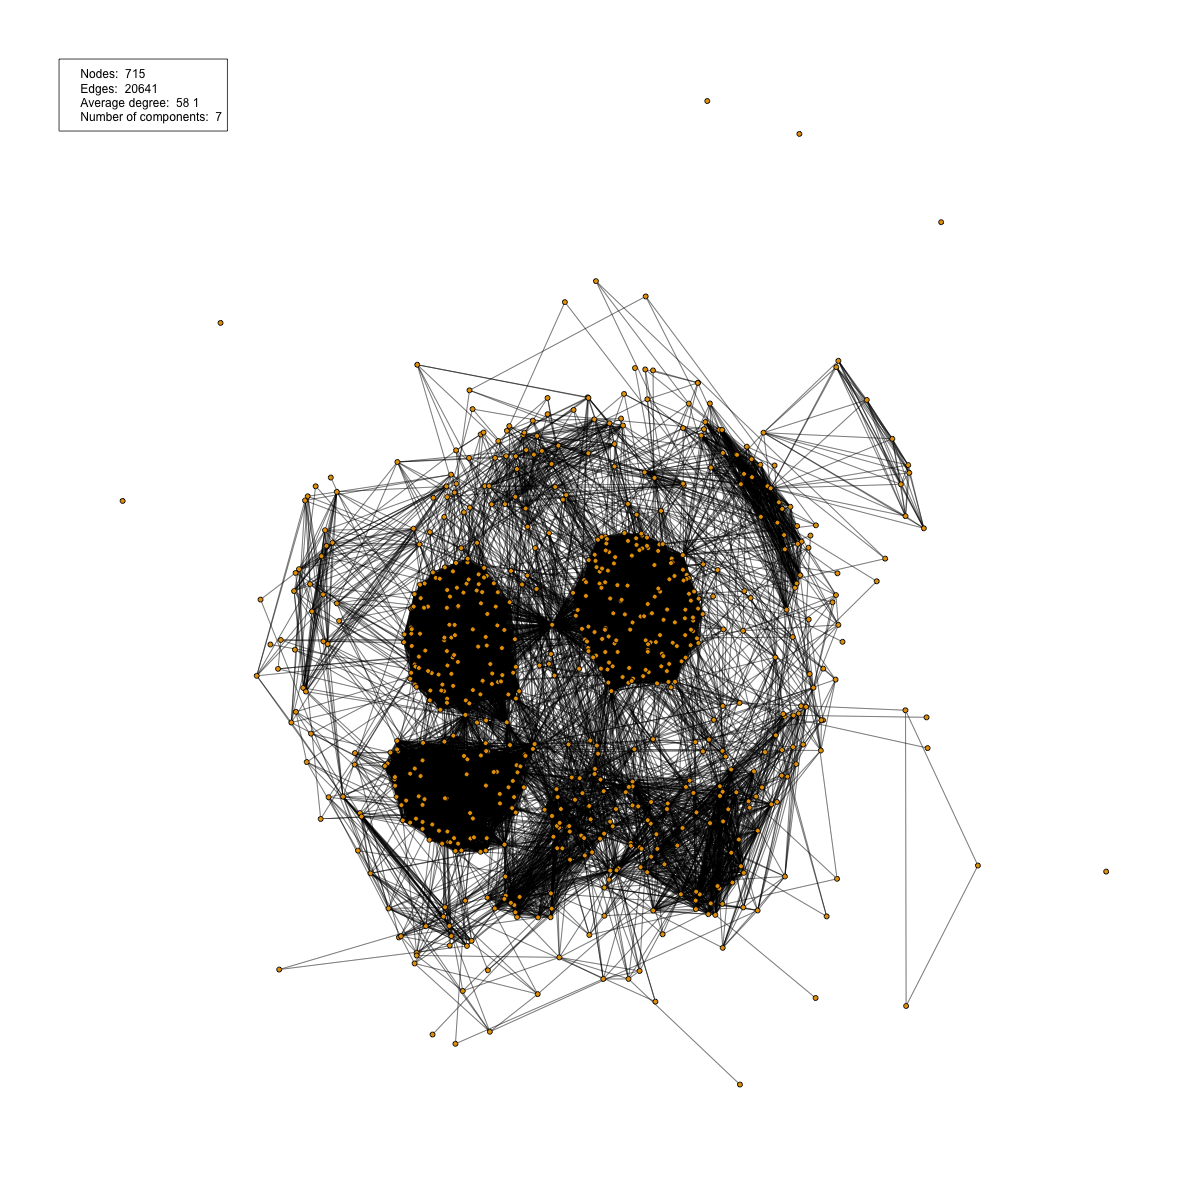
\includegraphics[width=14cm]{figures/graphs/cg_ln_mainnet_run1.png}
    \caption{Linked channels from LN mainnet run1}
    \label{fig:channelGraphLNTS}
\end{figure}

\begin{figure}[h]
    \centering
    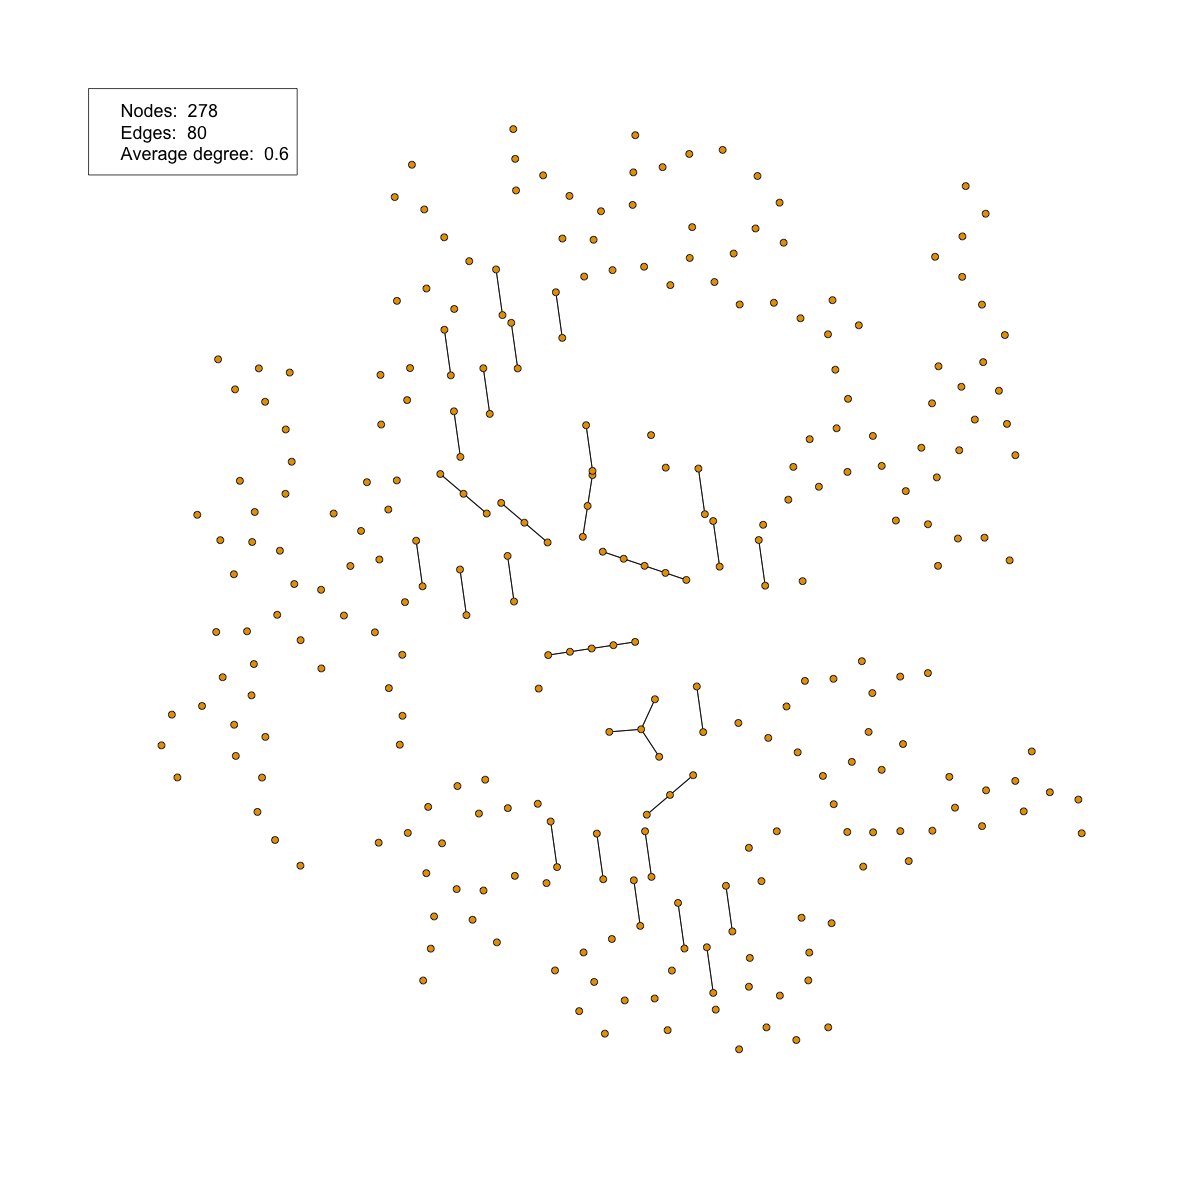
\includegraphics[width=14cm]{figures/graphs/cg_bc_mainnet_run1.png}
    \caption{Linked channels from BC mainnet run1}
    \label{fig:channelGraphLNTS}
\end{figure}
\chapter{Summary}
\label{chap:conclusion}

\section{Conclusion}
In this project we have explored the LN from the blockchain perspective.
As the LN does not change the Bitcoin system in any way, the older analysis methods are still valid if we don't consider the LN. Taking the LN into consideration means seeing transactions in the context of the LN in addition to the context of the blockchain. As we have discovered when attempting to locate on-chain LN transactions: one can never be perfectly sure that a transaction is LN related or not, if we only use the informatin available in the blockcahin. The different characteristics used to identify potential on-chain transactions have different level of uniqueness, but will limit the amount we can identify. Uniqueness makes it very unlikely that the transaction is not LN related, but as stated previously: users are free to create whichever scripts and transaction chains they wish. 
The identified channels does also contain limited amount of information allowing us to infer things about the LN, especially in terms of off-chain transaction. As the on-chain transactions facilities the channels in the LN, most of the information we get are related to these and its users.
While this information might allow for us to determine some of the structure of the LN, in terms of which channels are connected, it does not in our opinion help in determining anything about potential off-chain transaction flows. We can therefore conclude, from the blockchain analysis perspective, that doing transfers within the LN provides much better privacy than doing transfers on-chain.
\\


% identification
Our results also show some possibilities. In our second interval comparing the channels found with our two methods of identification, and channels collected trough the LN, we see that possibly more than 75\% of all 2of2 multisig transactions is in fact LN channels. This was due to the possible limits of our LN node to collect all channels, as other nodes will remove inactive channels and they will therefore not be propagated. This might become apparent if one where to use longer collection intervals, or run the collection node longer before starting to collect, allowing the node to receive many channels will eventually be pruned by other nodes.
The timelocked identification provides a good middle ground between precision and how many channels it will be able to find, with the results from the second interval indicating that around 25\% of channels is unilaterally closed. As shown in our correlation between P2WSH outputs and number of channels on the LN, the P2WSH outputs can be used as an indicator of the number of channels, but at least providing a upper limit on active channels at any point in time. It is important to note however that these things are very reliant on the current use cases of the things used for identification and correlation. For example, if 2of2 multisig is used commonly for other things than LN channels, identification based on it will become extremely unreliable. 
\\


% linking
As the linking done between identified channels only utilized information found within the channel graphs themselves. We should take note that much of the principles for linking information on the blockchain is still relevant for this case. Using new keys for each transaction giving providing the users with pseudoanonymity is very much still relevant for channels graphs. In addition to enabling us to link channels containing the same keys, it will also enable linking of keys within the channel graph itself, which will make it easier to distinguish the users within the graph. As discussed previously, differentiating users within a graph would enable us to determine which users provide link between channels, allowing us to recreate parts of the structure of the LN more accurately. But when attempting to link keys within a channel graph, the entire transaction graph should also be used, linking all possible keys. Our linking results show that the information available and our heuristics are very limited. When comparing the channel network created by using information from the LN, with the one created using channel graphs found in the blockchain in the same interval, we can see a very clear difference in the number of edges. The network using LN information has a average degree over a hundred times larger than the channel network from the blockchain. The effectiveness of our heuristics is dependent on user behaviour, and how LN implementations operates in regard to transaction structure. For example, using a single transaction to spend many timelocked outputs is simple and convenient, but allows for linking using our third heuristic.
\\


It is apparent that if one wants information about the LN, it is in most cases better to simply get this directly from the LN, instead of finding it on the blockchain.
But as we previously have pointed out: all LN channels needs to be anchored on the blockchain, which contains verified historical data, so it will be a important source of information with regards to the LN. 
Additionally, blockchain analysis can be used in conjunction with other methods of analysis on the LN, providing a supplement. 

\section{Future Work}
\label{sec:future}

As a emerging technology the LN and Bitcoin system is being changed and improved regularly, and because the work presented here is for the current state of these systems, any future work using elements from this project, will have to change methods and assumptions.
A example is founding transactions: currently founding transactions can be used to found a single channel, but there is nothing in the way of having a single founding transaction for many channels \cite{multi_channel_founding}.
This would provide additional possibilities for linking.
It could also be used for identification of channels-e.g., one channel might be identified because of a timelocked output, and by finding ouputs of other channels in the founding transaction we can also identify them.
\\

One of the proposed improvements that will impact this type of work the most is channel factories \cite{burchert2017scalable}.
The proposition is to have a additional layer between the blockchain and the payment channel network, with the purpose of creating the one-to-one payment channels which makes up the payment channel network.
The channel factories on this layer can manage channels, meaning payment channels no longer requires any on-chain transactions to manage.
The channel factories itself requires on-chain transactions, but with such a additional layer of abstraction, allowing for many dynamic channels per on-chain transactions, the use and methods of blockchain analysis must be reassessed.
\\


\ifthenelse{\boolean{HarvardCitations}}{%
	\bibliographystyle{agsm} % used for Harvard style references. Names - Humanities & Interaction Design
}{%
	\bibliographystyle{ntnuthesis/ntnuthesis} %used for Vancover style references. Numbers - Computer Science & Physics
}

\bibliography{refs}

\appendix
\chapter{Appendix}

\section{Additional channel networks}
\label{appendix_networks}

\subsection{Second interval mainnet}

\begin{figure}[ht]
    \centering
    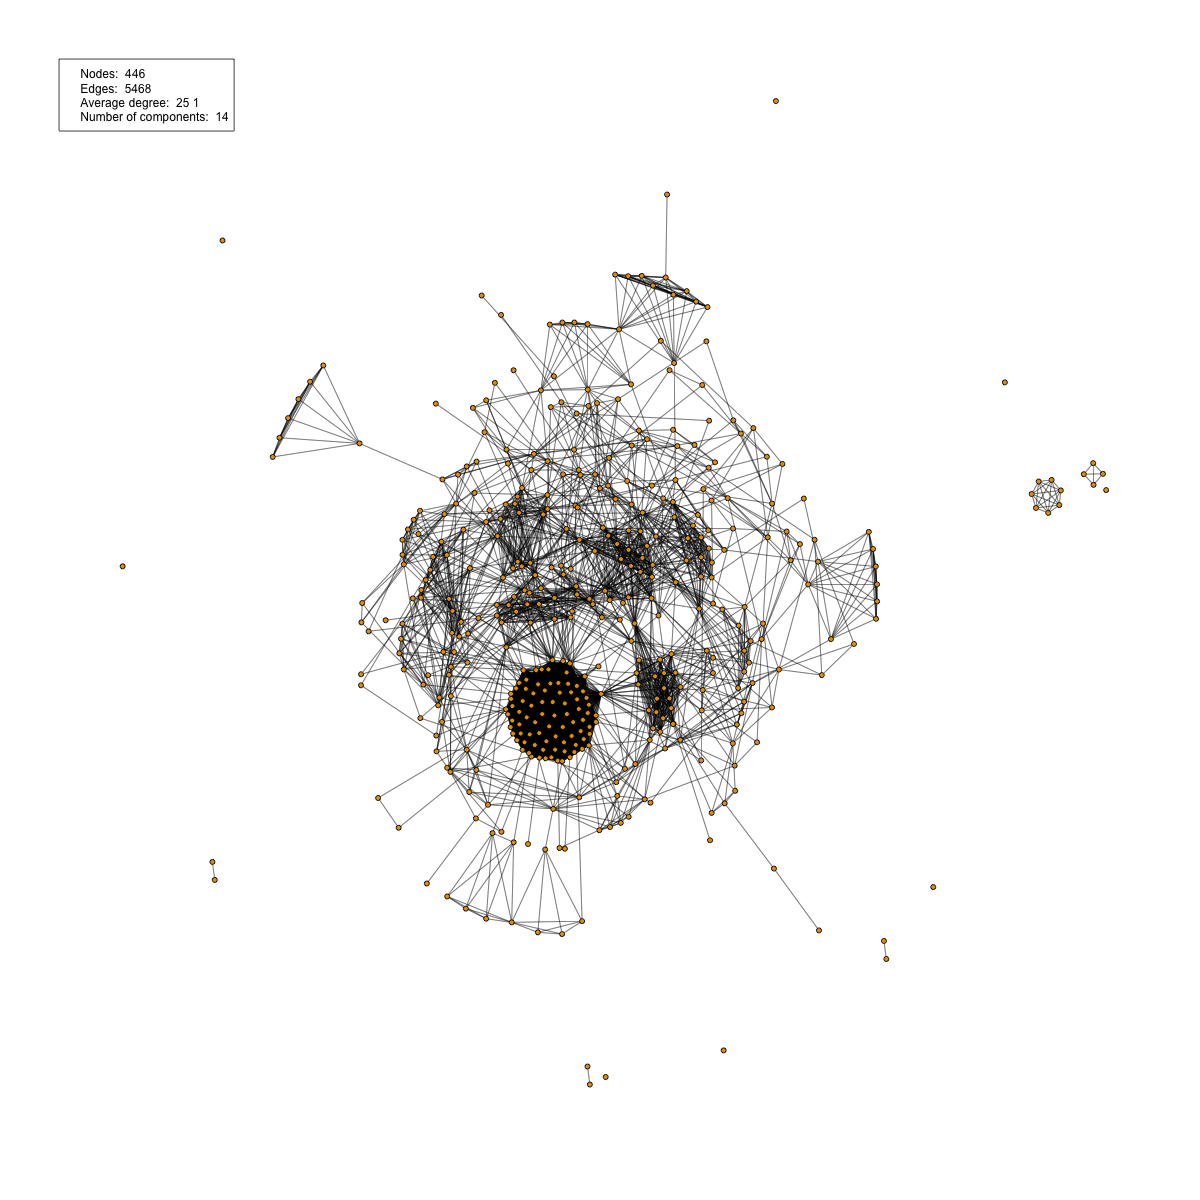
\includegraphics[width=14cm]{figures/graphs/cg_ln_mainnet_run2.png}
    \caption{Channel network from the LN, mainnet, second interval}
    \label{fig:channel_network_LN_mainent2}
\end{figure}

\begin{figure}[H]
    \centering
    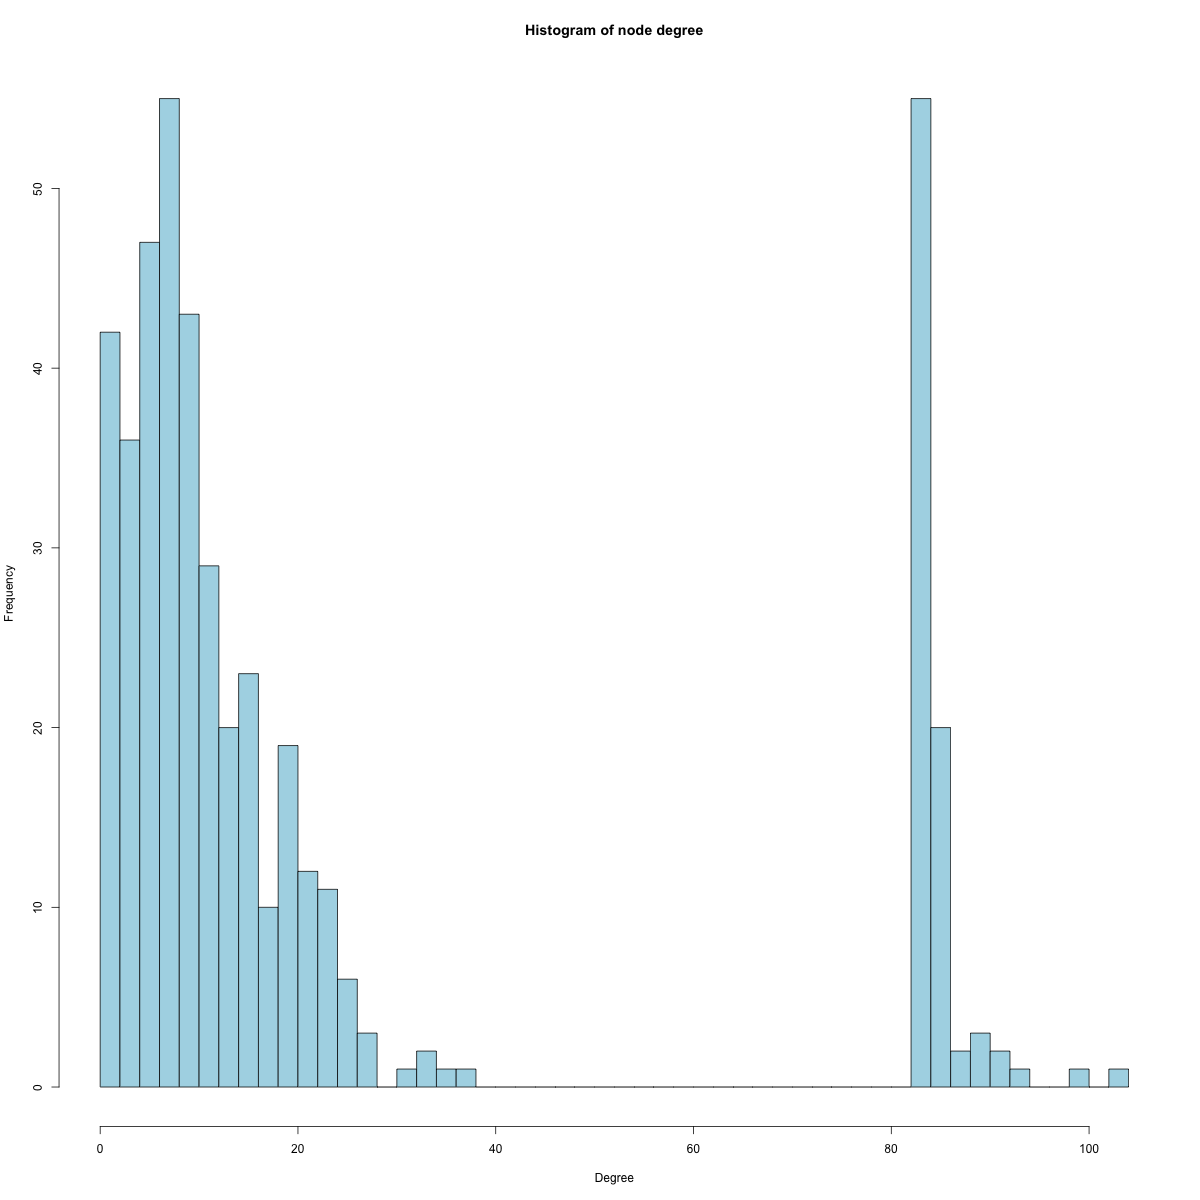
\includegraphics[width=16cm]{figures/graphs/histogram_ln_mainnet_run2.png}
    \caption{Histogram of node degree for the network in \cref{fig:channel_network_LN_mainent2}}
    \label{fig:histogram}
\end{figure}

\begin{figure}[H]
    \centering
    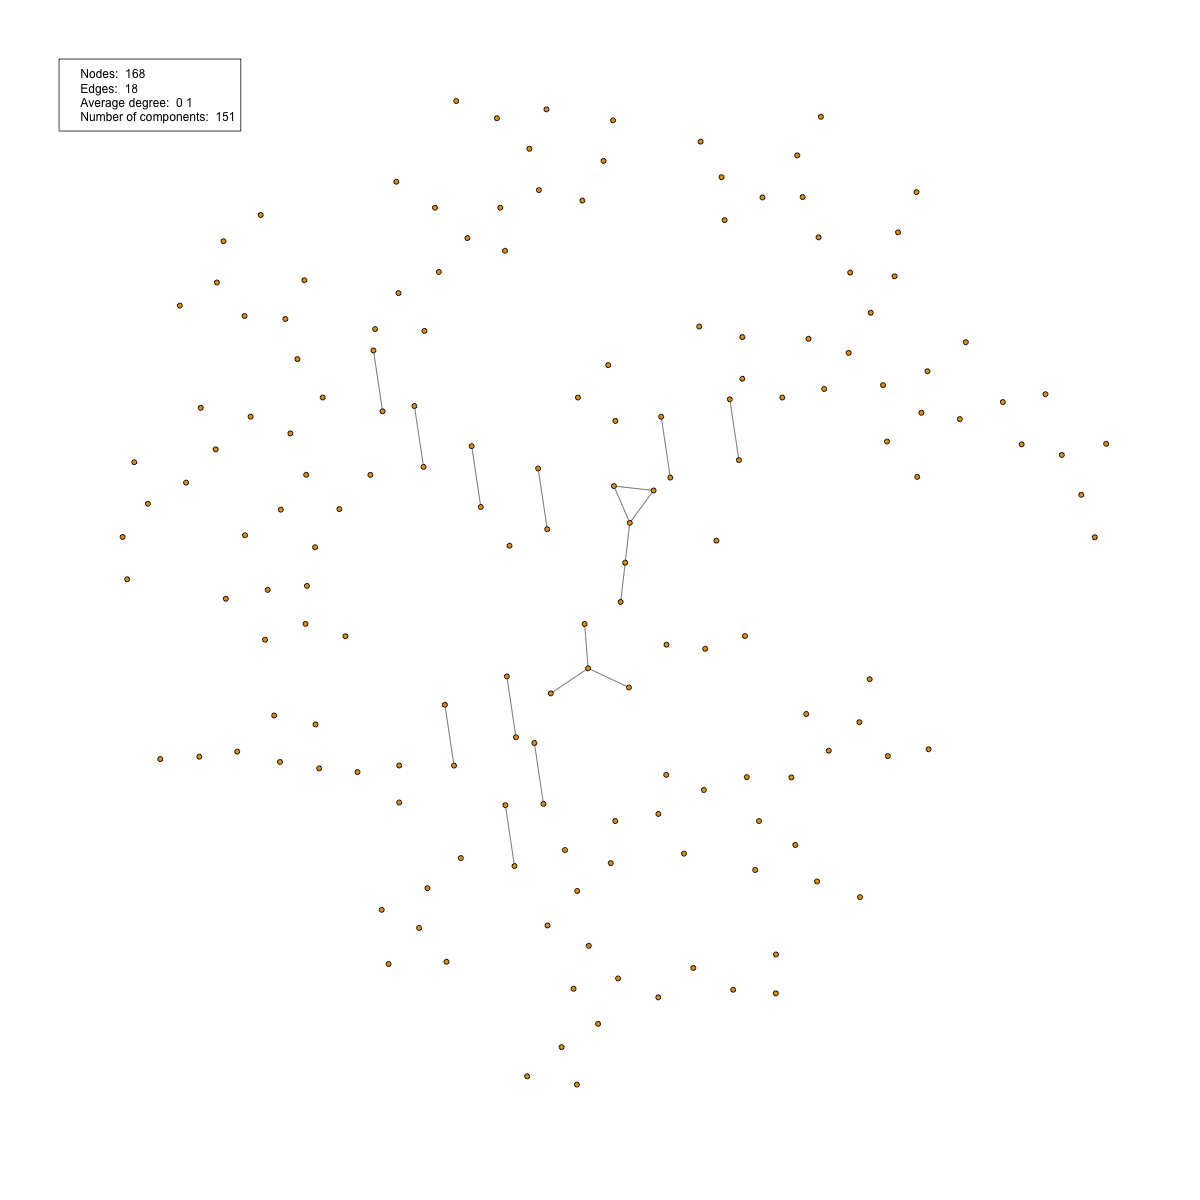
\includegraphics[width=14cm]{figures/graphs/cg_bc_mainnet_run2.png}
    \caption{Channel network from the blockchain, mainnet, second interval}
    \label{fig:channel_network_BC_mainnet}
\end{figure}


\subsection{Testnet}

\begin{figure}[ht]
    \centering
    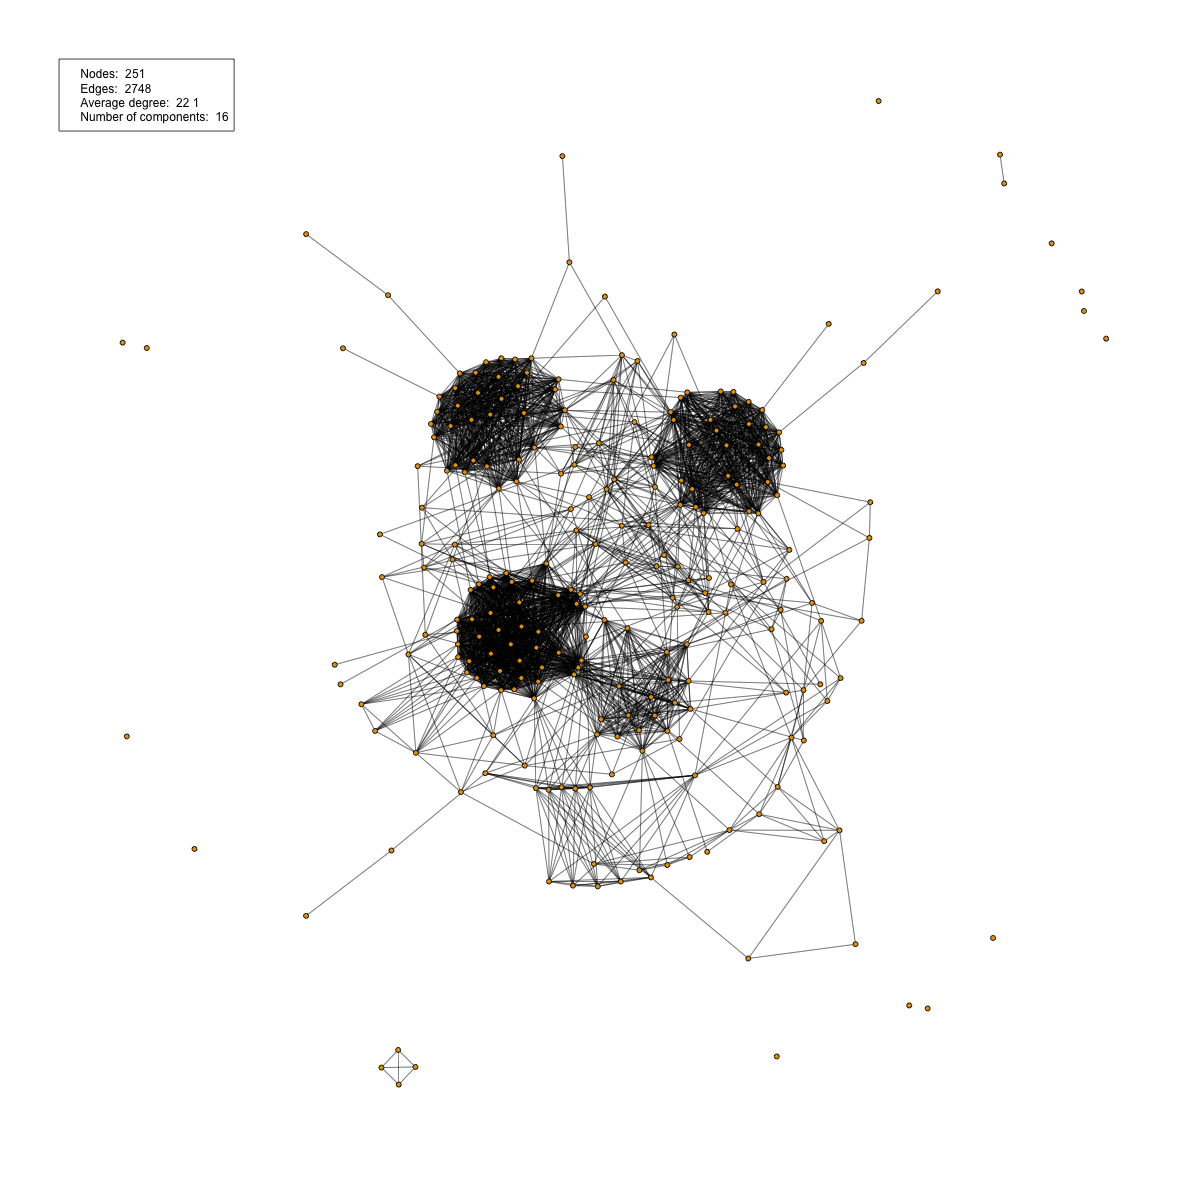
\includegraphics[width=14cm]{figures/graphs/cg_ln_testnet_run1.png}
    \caption{Channel network from the LN testnet, from interval one}
    \label{fig:channel_network_LN_testnet}
\end{figure}

\begin{figure}[H]
    \centering
    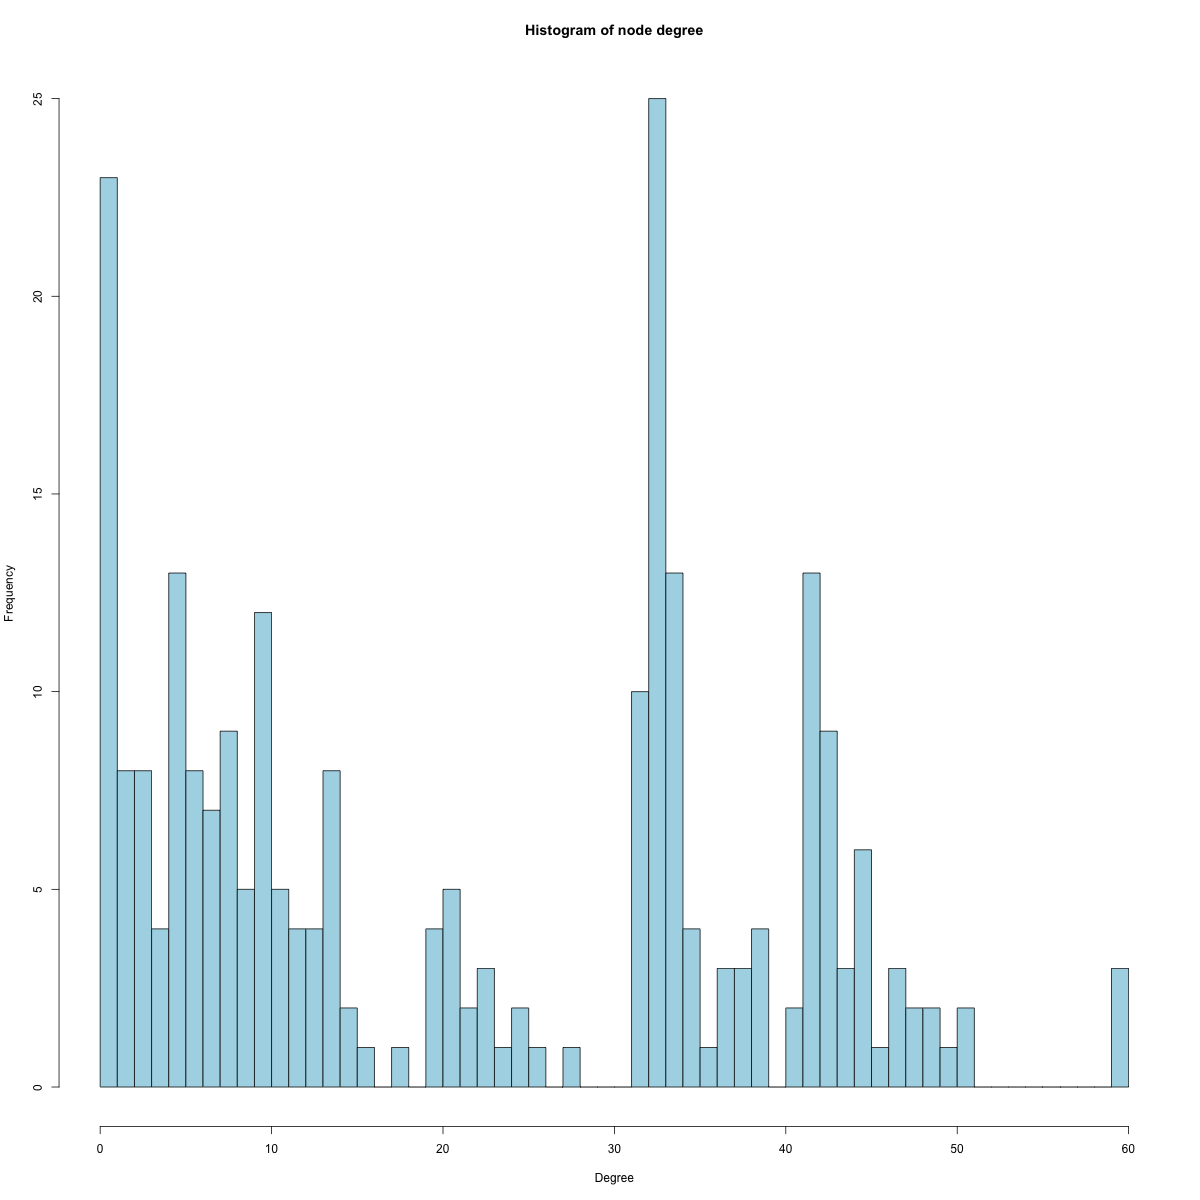
\includegraphics[width=16cm]{figures/graphs/histogram_ln_testnet_run1.png}
    \caption{Histogram of node degree for the network in \cref{fig:channel_network_LN_testnet}}
    \label{fig:histogram}
\end{figure}

\begin{figure}[H]
    \centering
    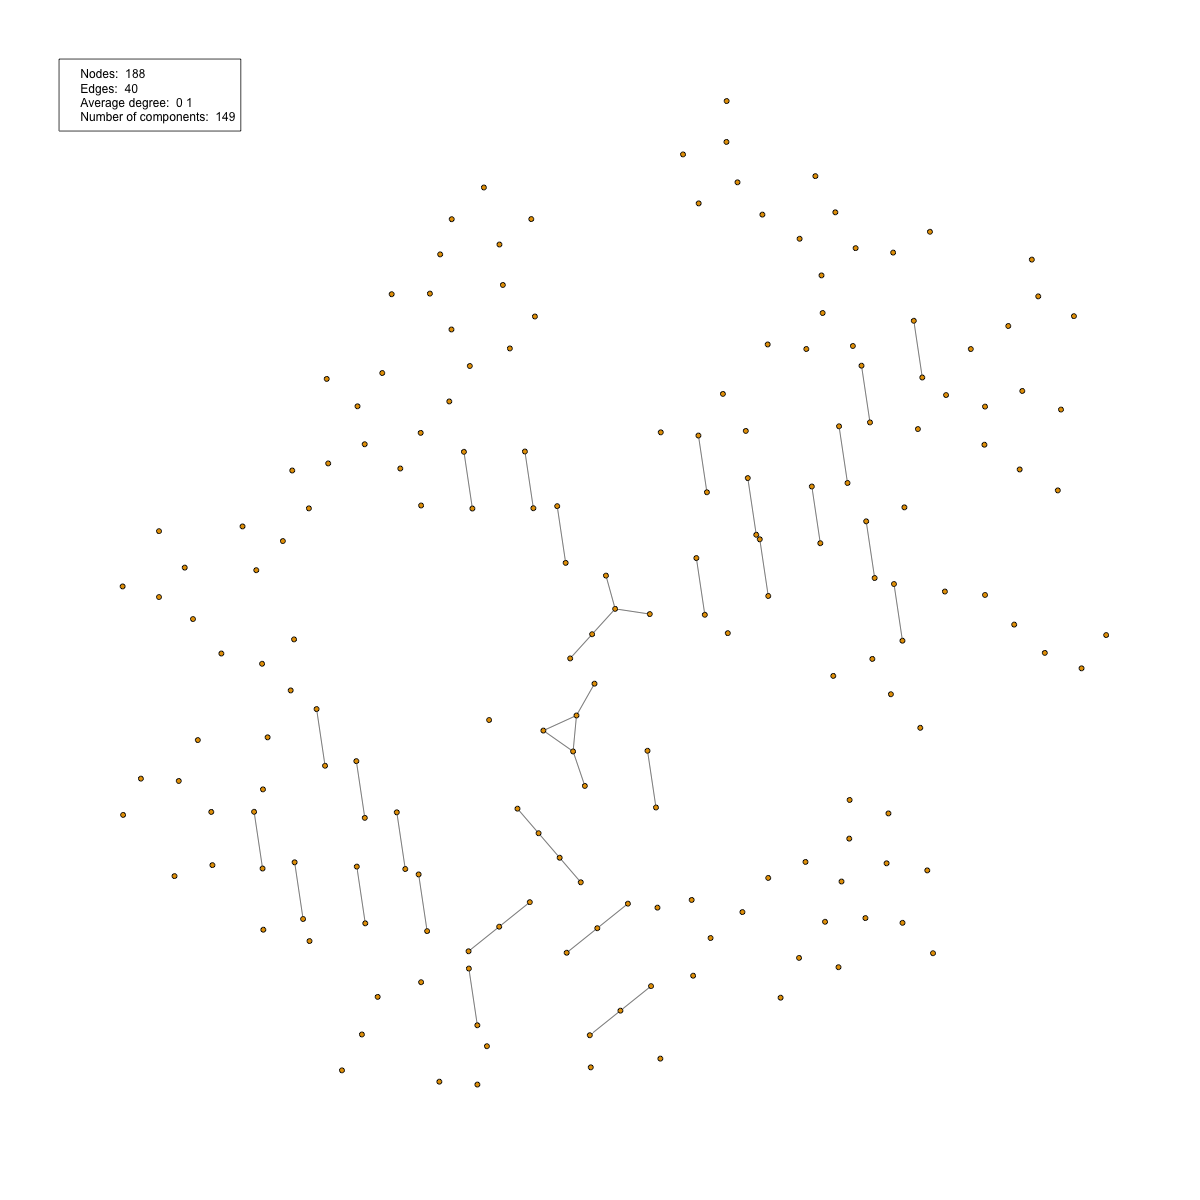
\includegraphics[width=14cm]{figures/graphs/cg_bc_testnet_run1.png}
    \caption{Channel network from the testnet blockchain, from interval one}
    \label{fig:channel_network_BC_testnet}
\end{figure}

%\include{inc/timetable}

\end{document}
